\documentclass[11pt, a4paper]{article}
\setlength{\headheight}{13.6pt}

% ── Encoding & language ───────────────────────────────────────────────────────
\usepackage[T1]{fontenc}
\usepackage[utf8]{inputenc}
\usepackage[english]{babel}

% ── Fonts & micro-typography ──────────────────────────────────────────────────
\usepackage{lmodern}
\usepackage{microtype}

% ── Math ──────────────────────────────────────────────────────────────────────
\usepackage{amsmath, amssymb, amsthm}
\usepackage{mathtools}

% ── Algorithms ────────────────────────────────────────────────────────────────
\usepackage{algorithm}
\usepackage{algorithmic}

% ── Figures & tables ──────────────────────────────────────────────────────────
\usepackage{graphicx}
\usepackage{booktabs}
\usepackage{float}
\usepackage{caption}
\usepackage{subcaption}

% ── Code listings ─────────────────────────────────────────────────────────────
\usepackage{listings}
\usepackage{xcolor}
\lstset{
    language=Python,
    basicstyle=\small\ttfamily,
    numbers=left,
    numberstyle=\tiny,
    frame=single,
    breaklines=true,
    keywordstyle=\color{blue!70!black},
    commentstyle=\color{green!50!black},
    stringstyle=\color{orange!80!black},
}

% ── Hyperlinks (must come before cleveref) ────────────────────────────────────
\usepackage{hyperref}
\hypersetup{
    colorlinks = true,
    linkcolor  = blue!60!black,
    citecolor  = blue!60!black,
    urlcolor   = blue!60!black,
    pdftitle   = {SF1546 Project VT2026},
}

% ── Cross-referencing (after hyperref) ───────────────────────────────────────
\usepackage[capitalise, noabbrev]{cleveref}
% Tell cleveref how to name listing floats
\crefname{lstlisting}{Listing}{Listings}
\Crefname{lstlisting}{Listing}{Listings}

% ── Page geometry ─────────────────────────────────────────────────────────────
\usepackage{geometry}
\geometry{margin=2cm}

% ── Header / footer ───────────────────────────────────────────────────────────
\usepackage{fancyhdr}
\pagestyle{fancy}
\fancyhf{}
\lhead{SF1546 -- Project VT2026}
\rhead{Group 41}
\cfoot{\thepage}
\setlength{\parindent}{0pt}
% ── Theorem-like environments ─────────────────────────────────────────────────
\newtheorem{theorem}{Theorem}
\newtheorem{lemma}[theorem]{Lemma}
\newtheorem{corollary}[theorem]{Corollary}
\newtheorem{proposition}[theorem]{Proposition}
\theoremstyle{definition}
\newtheorem{definition}[theorem]{Definition}
\newtheorem{remark}[theorem]{Remark}

% ── Useful macros ─────────────────────────────────────────────────────────────
\newcommand{\dif}{\mathop{}\!\mathrm{d}}
\newcommand{\Ord}[1]{\mathcal{O}\!\left(#1\right)}
\newcommand{\norm}[1]{\left\lVert#1\right\rVert}

% ══════════════════════════════════════════════════════════════════════════════
\begin{document}

% ── Title page ────────────────────────────────────────────────────────────────
\begin{titlepage}
  \centering
  \vspace*{1.5cm}
  {\Large KTH -- School of Engineering Sciences (SCI)\par}
  \vspace{0.4cm}
  {\large SF1546 Numerical Methods, Basic Course\par}
  \vspace{2cm}
  {\huge\bfseries Heat Transfer: From Theory to Numerical Solutions\par}
  \vspace{0.8cm}
  {\Large Project VT2026\par}
  \vspace{3cm}

  \begin{tabular}{@{}lcl@{}}
    \toprule
    \textbf{Name} & \textbf{Personal ID} & \textbf{E-mail} \\
    \midrule
    lastname, firstnamt & 12345 & \texttt{mymail@kth.se} \\
    \bottomrule
  \end{tabular}

  \vspace{1.5cm}
  {\large Group 41\par}
  \vspace{0.5cm}
  {\large \today\par}
\end{titlepage}

% ── Table of contents ─────────────────────────────────────────────────────────
\tableofcontents
\newpage

% ══════════════════════════════════════════════════════════════════════════════
\section{Introduction}
In modern engineering we are often faced with challenges of optimization, whether they are about minimizing cost or maximizing efficiency each case relies on mathematical models to try and predict a systems behaviour. In the first part of this report we analyse a heat exchanger which has a range of parameters already set and attempt to find optimal geometric parameters that satisfies the specifications. We do this by showing how the problem can be converted into a \textit{root finding problem} and solved using Newton's Method with python code. Furthermore, we verify that our solution is reasonable by comparing it to theoretical expectations of such an implementation as well as comparing results with those obtained using established libraries such as scipy.

The second part of the report is spent on modelling a one-dimensional heat sink and it's thermal diffusion properties relating to choice of material and size. We show, in a similar way to the heat exchange model, how this boundary value problem can be formulated as a system of equations and solved using finite differences approximation and Newton's Method. The results are compared to a analytical case where simplifications to the model are made such that we can find an analytical solution to the governing equation and calculate an approximate error with which we can determine the models order of accuracy and when this analytical approximation makes sense. Finally we evaluate three materials with different thermal properties and assert a optimal length and choice of material for the heat sink.
% ══════════════════════════════════════════════════════════════════════════════
\section{Method}
\subsection{Part 1 -- Heat Exchanger}
We are tasked with determining a numerical value of the \textit{maximum} outer
tube diameter $d$ that simultaneously fulfills the specification of the other
parameters given below. An equation for the heat flux is given by \cref{eq:Q}.

\begin{equation}
  Q = A_{\mathrm{ex}} \cdot U_f \cdot \Delta T_m,
  \label{eq:Q}
\end{equation}

where $Q = 801368\ \mathrm{W}$ is the total heat flux,
$A_{\mathrm{ex}} = 64.15\ \mathrm{m}^2$ is the heat transfer area,
$\Delta T_m = 29.6\ ^\circ\mathrm{C}$ is the mean temperature difference
between the two fluids, and $U_f$ is the overall heat transfer coefficient
given by

\begin{equation}
  U_f = \left(
    \frac{d}{D_s h_t}
    + \frac{d R_{fi}}{D_s}
    + \frac{d \ln(d/D_s)}{2k_w}
    + R_{fo} + \frac{1}{h_s}
  \right)^{-1}.
  \label{eq:Uf}
\end{equation}
Here, $d$ is the outer tube diameter which is as of yet undefined and, $D_s = 1.219\ \mathrm{m}$
is the inner shell diameter, $R_{fi}$, $R_{fo}$, $h_s$, $h_t$, $k_w$ are
material and thermodynamic parameters given in \cref{tab:params1}.

\begin{table}[H]
  \centering
  \begin{tabular}{@{}ccc@{}}
    \toprule
    Parameter & Value & Unit \\
    \midrule
    $R_{fi}$ & $1.76 \cdot 10^{-4}$ & $\dfrac{\mathrm{m}^2\,{^\circ}\mathrm{C}}{\mathrm{W}}$ \\[10pt]
    $R_{fo}$ & $1.76 \cdot 10^{-4}$ & $\dfrac{\mathrm{m}^2\,{^\circ}\mathrm{C}}{\mathrm{W}}$ \\[10pt]
    $h_s$    & $356$                 & $\dfrac{\mathrm{W}}{\mathrm{m}^2\,{^\circ}\mathrm{C}}$ \\[10pt]
    $h_t$    & $356$                 & $\dfrac{\mathrm{W}}{\mathrm{m}^2\,{^\circ}\mathrm{C}}$ \\[10pt]
    $k_w$    & $60$                  & $\dfrac{\mathrm{W}}{\mathrm{m}\,{^\circ}\mathrm{C}}$   \\[6pt]
    \bottomrule
  \end{tabular}
  \caption{Parameter values.}
  \label{tab:params1}
\end{table}

% ············································································
\subsubsection{Newton's Method for a Non-Linear Equation}

To find a numerical value for $d$ we apply Newton's method for scalar problems
programmatically as outlined in \cref{alg:newton_scalar}.

\begin{algorithm}[H]
  \caption{Newton's method -- scalar equation}
  \label{alg:newton_scalar}
  \begin{algorithmic}
    \STATE{Let the initial guess be $d_0$ and the tolerance $\varepsilon$}
    \STATE{$k \leftarrow 0$}
    \WHILE{$|f(d_k)| > \varepsilon$}
      \STATE{$d_{k+1} \leftarrow d_k - f(d_k)/f'(d_k)$}
      \STATE{$k \leftarrow k+1$}
    \ENDWHILE
    \STATE{\textbf{return} $d_k$}
  \end{algorithmic}
\end{algorithm}

We must therefore first find our function $f(d_k)$ on which we can apply Newton's method.
We begin by rearranging \cref{eq:Q} into:

\begin{equation}
    U_f = \frac{Q}{A_{\mathrm{ex}}\cdot \Delta T_m},
    \label{eq:U_f2}
\end{equation}

Newton's method is a \textit{root finding} algorithm and as such solves
$f(d_k) = 0$ by definition. We therefore subtract \cref{eq:U_f2} from
\cref{eq:Uf} and arrive at our expression for $f(d_k)$:

\begin{equation}
    f(d_k) = \left(
    \frac{d_k}{D_s h_t}
    + \frac{d_k R_{fi}}{D_s}
    + \frac{d_k \ln(d_k / D_s)}{2k_w}
    + R_{fo} + \frac{1}{h_s}
  \right)^{-1} - \frac{Q}{A_{\mathrm{ex}}\cdot \Delta T_m} = 0
    \label{eq:f(d)}
\end{equation}

Taking the derivative with respect to $d$, our second term vanishes.
Applying the chain rule:

\begin{equation}
    \frac{\dif}{\dif d_k} f(d_k) = f'(d_k) =
    -\frac{
        \dfrac{1}{D_s h_t} + \dfrac{R_{fi}}{D_s} + \dfrac{\ln(d_k/D_s) + 1}{2k_w}
    }{
        \left(
            \dfrac{d_k}{D_s h_t}
            + \dfrac{d_k R_{fi}}{D_s}
            + \dfrac{d_k \ln(d_k/D_s)}{2k_w}
            + R_{fo} + \dfrac{1}{h_s}
        \right)^{2}
    }
    \label{eq:f'(d)}
\end{equation}

We can now assemble the final expression for Newton's Method, the update is given by:

\begin{equation}
    d_{k+1} = d_k - \frac{f(d_k)}{f'(d_k)}
    \label{eq:newtonsmethod}
\end{equation}

This is implemented and solved for using the python code in \cref{lst:NM-eq}.
% ══════════════════════════════════════════════════════════════════════════════

\subsubsection{Newton's Method for a Non-linear System of Equations}

We must now also consider the pressure drop $\Delta P$ and surface area of heat transfer $A_{ex}$ as functions of the inner shell diameter $D_s$ in our system along with the added restriction that the \textit{maximum} $\Delta P$ allowed is $49080\ \mathrm{Pa}$. We must therefore now move to solving a \textit{system} of equations since $\Delta P$ and $A_{ex}$ are expressed with \cref{eq:Pdrop} and \cref{eq:Aex} respectively. \cref{tab:params2} give the parameter values for \cref{eq:Pdrop} and \cref{eq:Aex}.


\begin{equation}
    \Delta P = \frac{c}{D_s^2 (S_t - d)^2}
    \label{eq:Pdrop}
\end{equation}

\begin{equation}
    A_{ex} = \pi K_1 \frac{D_s^{n_1}}{d^{n_1-1}}
    \label{eq:Aex}
\end{equation}

\begin{table}[H]
  \centering
  \begin{tabular}{@{}ccc@{}}
    \toprule
    Parameter & Value & Unit \\
    \midrule
    $c$   & $0.389$ & $\mathrm{W\,s\cdot m}$ \\[6pt]
    $S_t$ & $0.016$ & $\mathrm{m}$ \\[6pt]
    $K_1$ & $0.249$ & $\mathrm{m}$ \\[6pt]
    $n_1$ & $2.207$ & $-$ \\[6pt]
    \bottomrule
  \end{tabular}
  \caption{Additional parameter values.}
  \label{tab:params2}
\end{table}
Since we now have to solve a system of equations for both the tube diameter $d$ as well as the inner shell diameter $D_s$ we move to Newton's Method for a \textit{system} of equations:
\begin{algorithm}[H]
  \caption{Newton's method -- system}
  \label{alg:newton_system}
  \begin{algorithmic}
    \STATE{Let the initial guess be $\mathbf{x}_0 = (d_0,\, D_{s,0})^T$ and tolerance $\varepsilon$}
    \STATE{$k \leftarrow 0$}
    \WHILE{$\|\mathbf{F}(\mathbf{x}_k)\| > \varepsilon$}
      \STATE{Solve $J\mathbf{F}(\mathbf{x}_k)\,\boldsymbol{\delta} = -\mathbf{F}(\mathbf{x}_k)$ for $\boldsymbol{\delta}$}
      \STATE{$\mathbf{x}_{k+1} \leftarrow \mathbf{x}_k + \boldsymbol{\delta}$}
      \STATE{$k \leftarrow k+1$}
    \ENDWHILE
    \STATE{\textbf{return} $\mathbf{x}_k = (d,\, D_s)^T$}
  \end{algorithmic}
\end{algorithm}

At each iteration, the linear system
$J\mathbf{F}(\mathbf{x}_k)\,\boldsymbol{\delta} = -\mathbf{F}(\mathbf{x}_k)$
is solved for the correction $\boldsymbol{\delta} = \mathbf{x}_{k+1} - \mathbf{x}_k$, which is then used to update the current guess. \\
We now formulate the Newton function $\mathbf{F}(d, D_s) = \mathbf{0}$ by
combining \cref{eq:Q,eq:Uf,eq:Aex,eq:Pdrop} into

\begin{equation}
  F_1(d, D_s) = \left(
      \frac{d}{D_s h_t} + \frac{d R_{fi}}{D_s}
      + \frac{d \ln(d/D_s)}{2k_w} + R_{fo} + \frac{1}{h_s}
    \right)^{-1}
    - \frac{Q\, d^{n_1-1}}{\pi K_1 D_s^{n_1} \Delta T_m}
  \label{eq:F1}
\end{equation}

\begin{equation}
  F_2(d, D_s) = \frac{c}{D_s^2(S_t - d)^2} - \Delta P
  \label{eq:F2}
\end{equation}
Combine into our Newton vector:
\begin{equation}
  \mathbf{F}(d, D_s) =
  \begin{pmatrix} F_1(d, D_s) \\ F_2(d, D_s) \end{pmatrix} = \mathbf{0},
  \quad \text{with } F_1, F_2 \text{ given by \cref{eq:F1,eq:F2}}
  \label{eq:system}
\end{equation}

To apply Newton's Method in higher dimensions we need the Jacobian $J\mathbf{F}$ which is computed analytically. Denoting
$g(d, D_s) = \frac{d}{D_s h_t} + \frac{d R_{fi}}{D_s}
+ \frac{d \ln(d/D_s)}{2k_w} + R_{fo} + \frac{1}{h_s}$
for brevity, the entries are:

\begin{equation}
  J\mathbf{F}(d, D_s) =
\begin{pmatrix}
  \partial_d F_1      & \partial_{D_s} F_1 \\[6pt]
  \partial_d F_2      & \partial_{D_s} F_2
\end{pmatrix}
  =
  \begin{pmatrix}
    -\dfrac{g_d}{g^2} + \dfrac{(n_1-1)Q\,d^{n_1-2}}{\pi K_1 D_s^{n_1} \Delta T_m}
    &
    \dfrac{g_{D_s}}{g^2} + \dfrac{n_1 Q\, d^{n_1-1}}{\pi K_1 D_s^{n_1+1} \Delta T_m}
    \\[12pt]
    \dfrac{2c}{D_s^2(S_t - d)^3}
    &
    \dfrac{-2c}{D_s^3(S_t - d)^2}
  \end{pmatrix}
  \label{eq:jacobian}
\end{equation}

Where $g_d = \partial g/\partial d$ and $g_{D_s} = \partial g / \partial D_s$ are:
\begin{align}
  g_d     &= \frac{1}{D_s h_t} + \frac{R_{fi}}{D_s} + \frac{\ln(d/D_s) + 1}{2k_w} \\[6pt]
  g_{D_s} &= -\frac{d}{D_s^2 h_t} - \frac{d R_{fi}}{D_s^2} - \frac{d}{2k_w D_s}
\end{align}

This system is then solved using the python code in \cref{lst:NM-sys}
\subsection{Part 2 - Heat Sinks}
For the second part we shift our focus to the dispersion of heat in a one-dimensional rod and study the governing equation, a case of the static heat equation:

\begin{equation}
\label{eq:heateq}
\frac{d^2T}{dx^2} = \alpha_1(T(x) -T_\infty) + \alpha_2f(T(x)), \quad 0\leq x  \leq L
\end{equation}
where $ f(t) = T^4(x) - T^4_\infty, \quad \alpha_1 = \frac{4 h_c}{DK}, \quad \alpha_2 = \frac{4 \epsilon \sigma}{DK}$ and our Dirichlet boundary conditions are $T(0) = T_s , \quad T(L) = T_L$. \footnote{See \cref{tab:3} for the constants.}

\subsubsection{Approximating the static heat equation}
Now, to be able to numerically solve \cref{eq:heateq} we apply the finite difference model, more specifically a central finite difference for the second derivative and solve for the temperature distribution $T(x)$ using Newtons method for a system of equations: \cref{alg:newton_system}. \\

For some second-order differential equation:
$$
\frac{d^2T}{dx^2} = \omega(x), \qquad \omega(x_j) = \omega_j, \quad x \in [0, L]
$$
a second-order central finite difference approximation is given by
$$
\frac{d^2T}{dx^2}\bigg|_{x_j}
\approx
\frac{T_{j+1} - 2T_j + T_{j-1}}{h^2}
+ \mathcal{O}(h^2).
$$
Where, for easier notation we let \( T(x_j) = T_j \). \newline
Divide the interval \([0,L]\) into $N$ sub intervals and let \(N=4\), so our grid points are
$$
j \in \{0,1,2,3,4\},
$$
with interior points \(j=1,2,3\). The step size is given by
$$
h = \frac{x_{end}-x_{start}}{N} = \frac{L-0}{4} = \frac{L}{4}.
$$
Therefore our points of evaluation becomes,
$$
x_0 = 0,\quad x_1 = h = \frac{L}{4},\quad x_2 = 2h = \frac{L}{2},\quad x_3 = 3h = \frac{3L}{4},\quad x_4 = 4h = L.
$$

Now, in our case as stated in \cref{eq:heateq}:
$$
\omega_j = \alpha_1\big(T(x_j) - T(\infty)\big) + \alpha_2 f\!\big(T(x_j)\big).
$$

Applying the approximation on each of the interior points we obtain a system of equations:
\[
\begin{cases}
\dfrac{T_2 - 2T_1 + T_0}{h^2}
=
\alpha_1\big(T_1 - T(\infty)\big) + \alpha_2 f(T_1), \\[6pt]
\dfrac{T_3 - 2T_2 + T_1}{h^2}
=
\alpha_1\big(T_2 - T(\infty)\big) + \alpha_2 f(T_2), \\[6pt]
\dfrac{T_4 - 2T_3 + T_2}{h^2}
=
\alpha_1\big(T_3 - T(\infty)\big) + \alpha_2 f(T_3).
\end{cases}
\]

applying the boundary conditions and moving the known boundaries to the right hand-side our system takes the form:
\[
\begin{cases}
\dfrac{T_2 - 2T_1}{h^2}
=
\alpha_1\big(T_1 - T(\infty)\big) + \alpha_2 f(T_1) - \dfrac{T_s}{h^2}, \\[6pt]
\dfrac{T_3 - 2T_2 + T_1}{h^2}
=
\alpha_1\big(T_2 - T(\infty)\big) + \alpha_2 f(T_2), \\[6pt]
\dfrac{T_2 - 2T_3}{h^2}
=
\alpha_1\big(T_3 - T(\infty)\big) + \alpha_2 f(T_3) - \dfrac{T_L}{h^2}.
\end{cases}
\]

Rewriting the system in compact matrix form, which can be generalized for an arbitrary $N$:
$$
A\mathbf{T} = \mathbf{r}(\mathbf{T}),
$$
where
$$
\mathbf{T} =
\begin{bmatrix}
T_1 \\[4pt]
T_2 \\[4pt]
T_3
\end{bmatrix},
\qquad
A =
\begin{bmatrix}
-2 & 1 & 0 \\[4pt]
1 & -2 & 1 \\[4pt]
0 & 1 & -2
\end{bmatrix},
$$
and
$$
\mathbf{r}(\mathbf{T}) =
\begin{bmatrix}
h^2\big[\alpha_1\big(T_1 - T(\infty)\big) + \alpha_2 f(T_1)\big] - T_s \\[6pt]
h^2\big[\alpha_1\big(T_2 - T(\infty)\big) + \alpha_2 f(T_2)\big] \\[6pt]
h^2\big[\alpha_1\big(T_3 - T(\infty)\big) + \alpha_2 f(T_3)\big] - T_L
\end{bmatrix}.
$$
\subsubsection{Solving the System}
\label{solving-the-system}
As for \cref{eq:system}, we apply Newton's method to our system, define the Newton function $\mathbf{F}(\mathbf{T})$:
$$
\mathbf{F}(\mathbf{T}) = A\mathbf{T} - \mathbf{r}(\mathbf{T}) = \mathbf{0}.
$$
Newton's method then solves
$$
\mathbf{J}_F(\mathbf{T})\,\boldsymbol{\delta} = -\mathbf{F}(\mathbf{T}),
$$
where the Jacobian is
$$
\mathbf{J}_F = \frac{\partial \mathbf{F}}{\partial \mathbf{T}} = A - \frac{\partial \mathbf{r}}{\partial \mathbf{T}}.
$$
and therefore:
$$
\mathbf{J}_F =
\begin{bmatrix}
-2 - h^2\big(\alpha_1 + \alpha_2 f'(T_1)\big) & 1 & 0 \\[6pt]
1 & -2 - h^2\big(\alpha_1 + \alpha_2 f'(T_2)\big) & 1 \\[6pt]
0 & 1 & -2 - h^2\big(\alpha_1 + \alpha_2 f'(T_3)\big)
\end{bmatrix}.
$$

With the code provided in \cref{lst:heatsinks} we then solve for the temperature distribution function $ \mathbf{T}(x) $.


% ══════════════════════════════════════════════════════════════════════════════
\section{Results}
\subsection{Part 1 -- Heat Exchanger}
% ············································································
\subsubsection{Numerical Solution of non-linear equation}
The implementation of Newton's Method on this problem using the Python-code in \cref{lst:NM-eq} produces the results shown in \cref{tab:newton_results}.
\begin{table}[h!]
\small
\centering
\begin{tabular}{cccccc}
\hline
\textbf{$d_0$ (mm)} & \textbf{$d^*$ (mm)} & \textbf{Iterations} & \textbf{$p$} & \textbf{Scipy $d^*$ (mm)} & \textbf{$|d^* - \text{Scipy}|$ (mm)} \\
\hline
  7.0000  &  19.131407149325682 & 3 & 2.332896 &  19.131407149308625 & $1.71\times 10^{-14}$ \\
 64.7500  &  19.131407149308647 & 4 & 2.322647 &  19.131407149308629 & $2.08\times 10^{-17}$ \\
122.5000  &  19.131407149308622 & 5 & 2.086488 &  19.131407149308611 & $1.04\times 10^{-17}$ \\
180.2500  &  19.131407151041735 & 5 & 1.850623 &  19.131407149308608 & $1.73\times 10^{-12}$ \\
238.0000  &  19.131407149308654 & 6 & 1.548516 &  19.131407149308618 & $3.82\times 10^{-17}$ \\
295.7500  &  19.131407149308636 & 6 & 1.058250 &  19.131407149308622 & $1.39\times 10^{-17}$ \\
\hline
353.5000  & 831.392740792126460 & 5 & 0.917235 & 831.392740793674875 & $1.55\times 10^{-12}$ \\
411.2500  & 831.392740793626103 & 7 & 1.350690 & 831.392740793672374 & $4.63\times 10^{-14}$ \\
469.0000  & 831.392740793674875 & 7 & 1.635620 & 831.392740793674761 & $1.11\times 10^{-16}$ \\
526.7500  & 831.392740791717188 & 6 & 1.774351 & 831.392740793674648 & $1.96\times 10^{-12}$ \\
584.5000  & 831.392740793674875 & 6 & 1.856506 & 831.392740793666690 & $8.22\times 10^{-15}$ \\
642.2500  & 831.392740791158303 & 5 & 1.911815 & 831.392740793674761 & $2.52\times 10^{-12}$ \\
700.0000  & 831.392740793674761 & 5 & 1.951238 & 831.392740793674761 & $0.00\times 10^{0}$ \\
\hline
\end{tabular}
\caption{Newton convergence results for all starting guesses $d_0$,
compared against \texttt{scipy.optimize.fsolve}. The horizontal rule separates
the two points of convergence: $d^* \approx 0.01913$ m and $d^* \approx 0.8314$ m.}
\label{tab:newton_results}
\end{table}

\cref{tab:newton_results} shows that the method, using the prescribed initial
guess $d_0 = 7.00\ \mathrm{mm}$, converges on a diameter of
$d_1^* \approx 19.13\ \mathrm{mm}$ after three iterations. Increasing the
initial guess in even increments reveals a \textit{second} root at
$d_2^* \approx 0.8314\ \mathrm{m}$, which is also evident from the plot of
$f(d)$ in \cref{fig:root_newton}. Since both these roots satisfy the heat transfer
specifications we opt for the larger outer tube diameter --- a larger tube diameter requires
fewer tubes for the same transfer area $A_\mathrm{ex}$, reducing both
material cost and manufacturing complexity.


The observed order of convergence $p$ varies across starting guesses but tend towards $p \approx 2$ as we approach a root, which is consistent with the theoretical \textit{local} quadratic convergence of Newton's method. Cases where $p$ deviates noticeably from the theoretical $p = 2$, such as at $d_0 = 353.5\,\mathrm{mm}$ with $p \approx 0.917$, can be attributed to starting values that lie far from a root and therefore outside the local neighbourhood where the quadratic convergence theorem applies.\footnote{A known limitation of Newton's Method is that one has to select an initial value that is already sufficiently close to a root for the method to be numerically stable.}
Inspecting Figure~\ref{fig:root_newton}, we see that the starting value $d_0 = 353.5\,\mathrm{mm}$ lies in a region where $f(d)$ is very steep and very far from both of the two roots. In this region, the tangent-based update
$$
d_{k+1} = d_k - \frac{f(d_k)}{f'(d_k)}
$$
has step length
$$
|d_{k+1} - d_k| = |- \frac{f(d_k)}{f'(d_k)}|
$$
and can produce updates with large steps that move far across the graph due the still very large function values before the iterates starts trending towards a specific root. In this initial phase, the error sequence is dominated by the global shape of $f(d)$ rather than its local quadratic behavior near the root, so the observed order of convergence is closer to linear than quadratic. This can be observed in \cref{fig:convergence} where the first step with starting guess $d_0 = 353.50 \ mm$ appears notably more linear than subsequent steps.


\begin{figure}[H]
    \centering
    \begin{minipage}{0.48\linewidth}
        \centering
        
\includegraphics[width=\linewidth]{Plots/outerdim_newton_roots.png}
        \caption{Graph of $f(d)$ over $d \in (0,\, 1]\ \mathrm{m}$, with the
        approximated roots marked.
        See \cref{lst:NM-eq} for the implementation.}
        \label{fig:root_newton}
    \end{minipage}
    \hfill
    \begin{minipage}{0.48\linewidth}
        \centering
        
\includegraphics[width=\linewidth]{Plots/outerdim_newton_convergence.png}
        \caption{Residual $|d_k - d^*|$ versus iteration $k$ for different starting guesses with Newton's method . See \cref{lst:NM-eq} \textit{"Order of Convergence"} section for implementation.}
        \label{fig:convergence}
    \end{minipage}
\end{figure}

% ──────────────────────────────────────────────────────────────────────────────
\subsubsection{Numerical Solution of the non-linear system}
Using the Python code in \cref{lst:NM-sys} we simultaneously solve for both the outer tube diameter $d$ and the inner shell diameter $D_s$ by implementing \cref{alg:newton_system}.
This code produces the results shown in \cref{tab:newton_sys:results}:

\begin{table}[h!]

\centering
\caption{Newton's Method for Nonlinear System $(d, D_s)$}
\label{tab:newton_sys:results}
\begin{tabular}{cccccc}
\hline
\textbf{$k$} & \textbf{$d_k$ (mm)} & \textbf{$D_{s,k}$ (mm)} & \textbf{$\lVert F(x_k)\rVert_2$} & \textbf{$\lVert x_k - x^*\rVert_2$} & \textbf{$p_k$} \\
\hline
 0  &  15.000000  & 800.000000  & $5.58732501\times 10^{5}$ & $1.15566350\times 10^{-1}$ & -- \\
 1  &  14.512150  & 777.419100  & $2.41670069\times 10^{5}$ & $9.29805713\times 10^{-2}$ & $0.262897$ \\
 2  &  13.883940  & 772.267000  & $9.65862053\times 10^{4}$ & $8.78141296\times 10^{-2}$ & $2.901072$ \\
 3  &  13.145660  & 758.858800  & $3.38316968\times 10^{4}$ & $7.43938660\times 10^{-2}$ & $2.157826$ \\
 4  &  12.479150  & 736.485600  & $8.77327269\times 10^{3}$ & $5.20133509\times 10^{-2}$ & $1.984354$ \\
 5  &  12.085780  & 710.043100  & $1.28077228\times 10^{3}$ & $2.55683086\times 10^{-2}$ & $1.531381$ \\
 6  &  11.942580  & 693.093400  & $1.09162252\times 10^{2}$ & $8.61795814\times 10^{-3}$ & $1.142165$ \\
 7  &  11.902210  & 686.964200  & $9.17536055\times 10^{0}$ & $2.48864323\times 10^{-3}$ & $1.023955$ \\
 8  &  11.891160  & 685.173200  & $1.00172096\times 10^{0}$ & $6.97587461\times 10^{-4}$ & $1.006337$ \\
 9  &  11.888110  & 684.669600  & $2.08936633\times 10^{-1}$ & $1.93969995\times 10^{-4}$ & $1.001770$ \\
10  &  11.887270  & 684.529400  & $5.62105801\times 10^{-2}$ & $5.38129237\times 10^{-5}$ & $1.000495$ \\
11  &  11.887030  & 684.490500  & $1.55480745\times 10^{-2}$ & $1.49197955\times 10^{-5}$ & $1.000138$ \\
12  &  11.886970  & 684.479700  & $4.30933832\times 10^{-3}$ & $4.13582602\times 10^{-6}$ & $1.000039$ \\
13  &  11.886950  & 684.476700  & $1.19450353\times 10^{-3}$ & $1.14640944\times 10^{-6}$ & $1.000015$ \\
14  &  11.886950  & 684.475900  & $3.31101187\times 10^{-4}$ & $3.17767263\times 10^{-7}$ & $1.000017$ \\
15  &  11.886950  & 684.475700  & $9.17765805\times 10^{-5}$ & $8.80783172\times 10^{-8}$ & $1.000052$ \\
16  &  11.886940  & 684.475600  & $2.54391336\times 10^{-5}$ & $2.44118045\times 10^{-8}$ & $1.000185$ \\
17  &  11.886940  & 684.475600  & $7.05135466\times 10^{-6}$ & $6.76437517\times 10^{-9}$ & $1.000667$ \\
18  &  11.886940  & 684.475600  & $1.95453191\times 10^{-6}$ & $1.87276678\times 10^{-9}$ & $1.002413$ \\
19  &  11.886940  & 684.475600  & $5.41767464\times 10^{-7}$ & $5.16884874\times 10^{-10}$ & $1.008796$ \\
20  &  11.886940  & 684.475600  & $1.50169740\times 10^{-7}$ & $1.41054272\times 10^{-10}$ & $1.032962$ \\
21  &  11.886940  & 684.475600  & $4.16249602\times 10^{-8}$ & $3.68797212\times 10^{-11}$ & $1.138833$ \\
22  &  11.886940  & 684.475600  & $1.15377952\times 10^{-8}$ & $8.00396433\times 10^{-12}$ & -- \\
23  &  11.886940  & 684.475600  & $3.19796218\times 10^{-9}$ & $0.00000000\times 10^{0}$ & -- \\
\hline
\end{tabular}
\end{table}

The method converges on values $d=11.886940\ mm$ and $D_s = 684.475600\ mm$ for the sought after diameters.
However, in the results we note that the order of convergence is not $p \approx 2$ as expected. Studying \cref{fig:NM.sys_loglog} and \cref{fig:convergence2} we conclude that the convergence appear linear instead of the theoretically expected quadratic behaviour. This is most likely due to the Jacobian being ill conditioned and close to singular near the solution.
\begin{figure}[H]
    \centering
    \begin{minipage}{0.48\linewidth}
        \centering
        
\includegraphics[width=\linewidth]{Plots/system_newton_loglog_errors.png}
        \caption{See \cref{lst:NM-sys} for the implementation.}
        \label{fig:NM.sys_loglog}
    \end{minipage}
    \hfill
    \begin{minipage}{0.48\linewidth}
        \centering
        
\includegraphics[width=\linewidth]{Plots/system_newton_residuals.png}
        \caption{Residual $|x_k - x^*|$ versus iteration $k$ for Newton's method. See \cref{lst:NM-sys} \textit{"Order of Convergence"} section for implementation.}
        \label{fig:convergence2}
    \end{minipage}
\end{figure}
% ············································································

\subsection*{Part 2 - Heat Sinks}
\subsubsection{Verification for the infinite length case}
To get some sense of whether or not our implementation seems reasonable, we test it against a case where the heat sink is so long that at some sufficiently large $x$ we expect the rod to reach ambient temperature $T_\infty$ and where radiative effects are neglected, this case has the analytical solution:

\begin{equation}
\label{eq:infty-analytical}
T(x) = T_\infty + (T_s - T_\infty)e^{-\sqrt{\alpha_1} x}.
\end{equation}

We use the values in \cref{tab:3} and approximate the temperature distribution function $T(x)$ for $N = 400 $ using the code in \cref{lst:heatsinks} and compare the results with \cref{eq:infty-analytical}, the results of which is shown in \cref{fig:heatsink-infty error} and \cref{fig:heatsink-inftyT}.

\begin{table}[h]
\centering
\caption{Heat Sink parameter values for implementation test.}
\label{tab:3}
\begin{tabular}{|c|c|c|}
\hline
\textbf{Parameter} & \textbf{Value} & \textbf{Unit} \\
\hline
$h_c$ & $40$ & $\dfrac{W}{m^2\cdot K}$ \\
\hline
$K$ & $240$ & $\dfrac{W}{m\cdot K}$ \\
\hline
$\epsilon$ & $0.4$ & \\
\hline
$\sigma$ & $5.67 \cdot 10^{-8}$ & $\dfrac{W}{m^2\,K^4}$ \\
\hline
$D$ & $4.13 \cdot 10^{-3}$ & $m$ \\
\hline
$T_s$ & $450$ & $K$ \, (Kelvin) \\
\hline
$T_\infty$ & $293$ & $K$ \, (Kelvin) \\
\hline
\end{tabular}
\end{table}

\begin{figure}[H]
    \centering
    \begin{minipage}{0.65\linewidth}
        \centering
        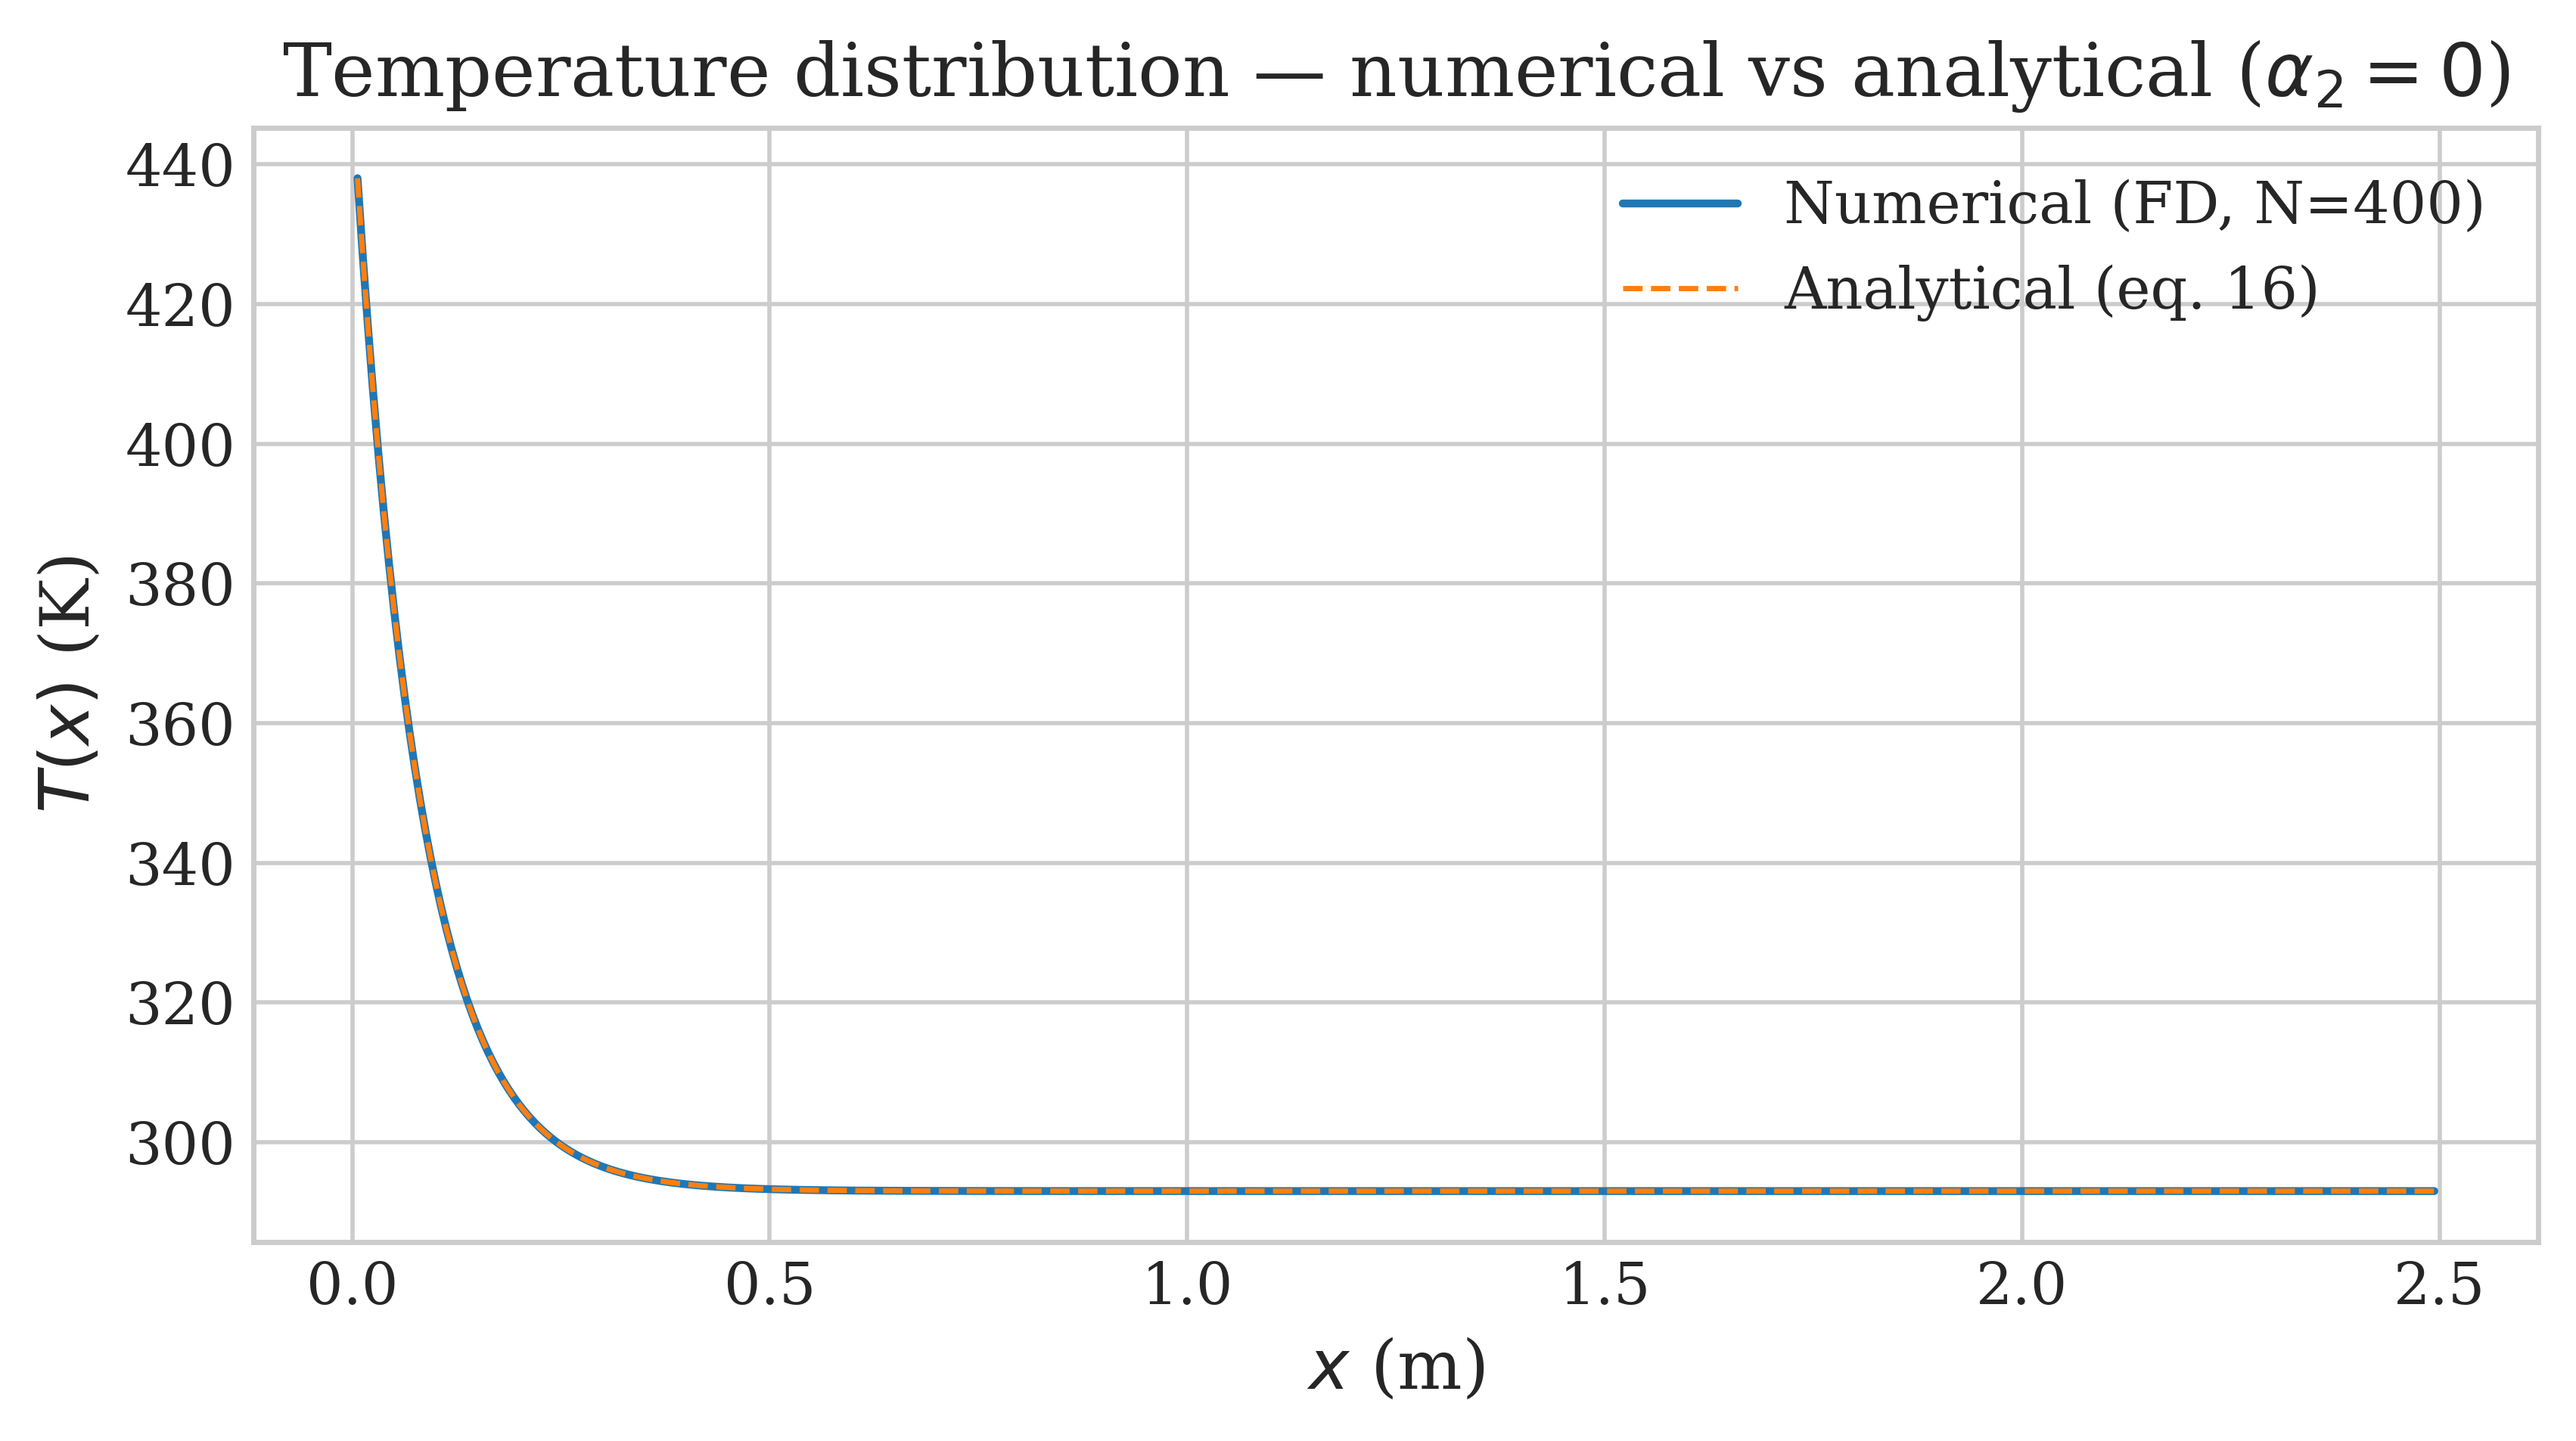
\includegraphics[width=\linewidth]{Plots/8_3a_solution.png}
        \caption{Temperature distribution of our approximate Newton solution compared to the analytical case \cref{eq:infty-analytical}}
        \label{fig:heatsink-inftyT}
    \end{minipage}
    \begin{minipage}{0.65\linewidth}
        \centering
        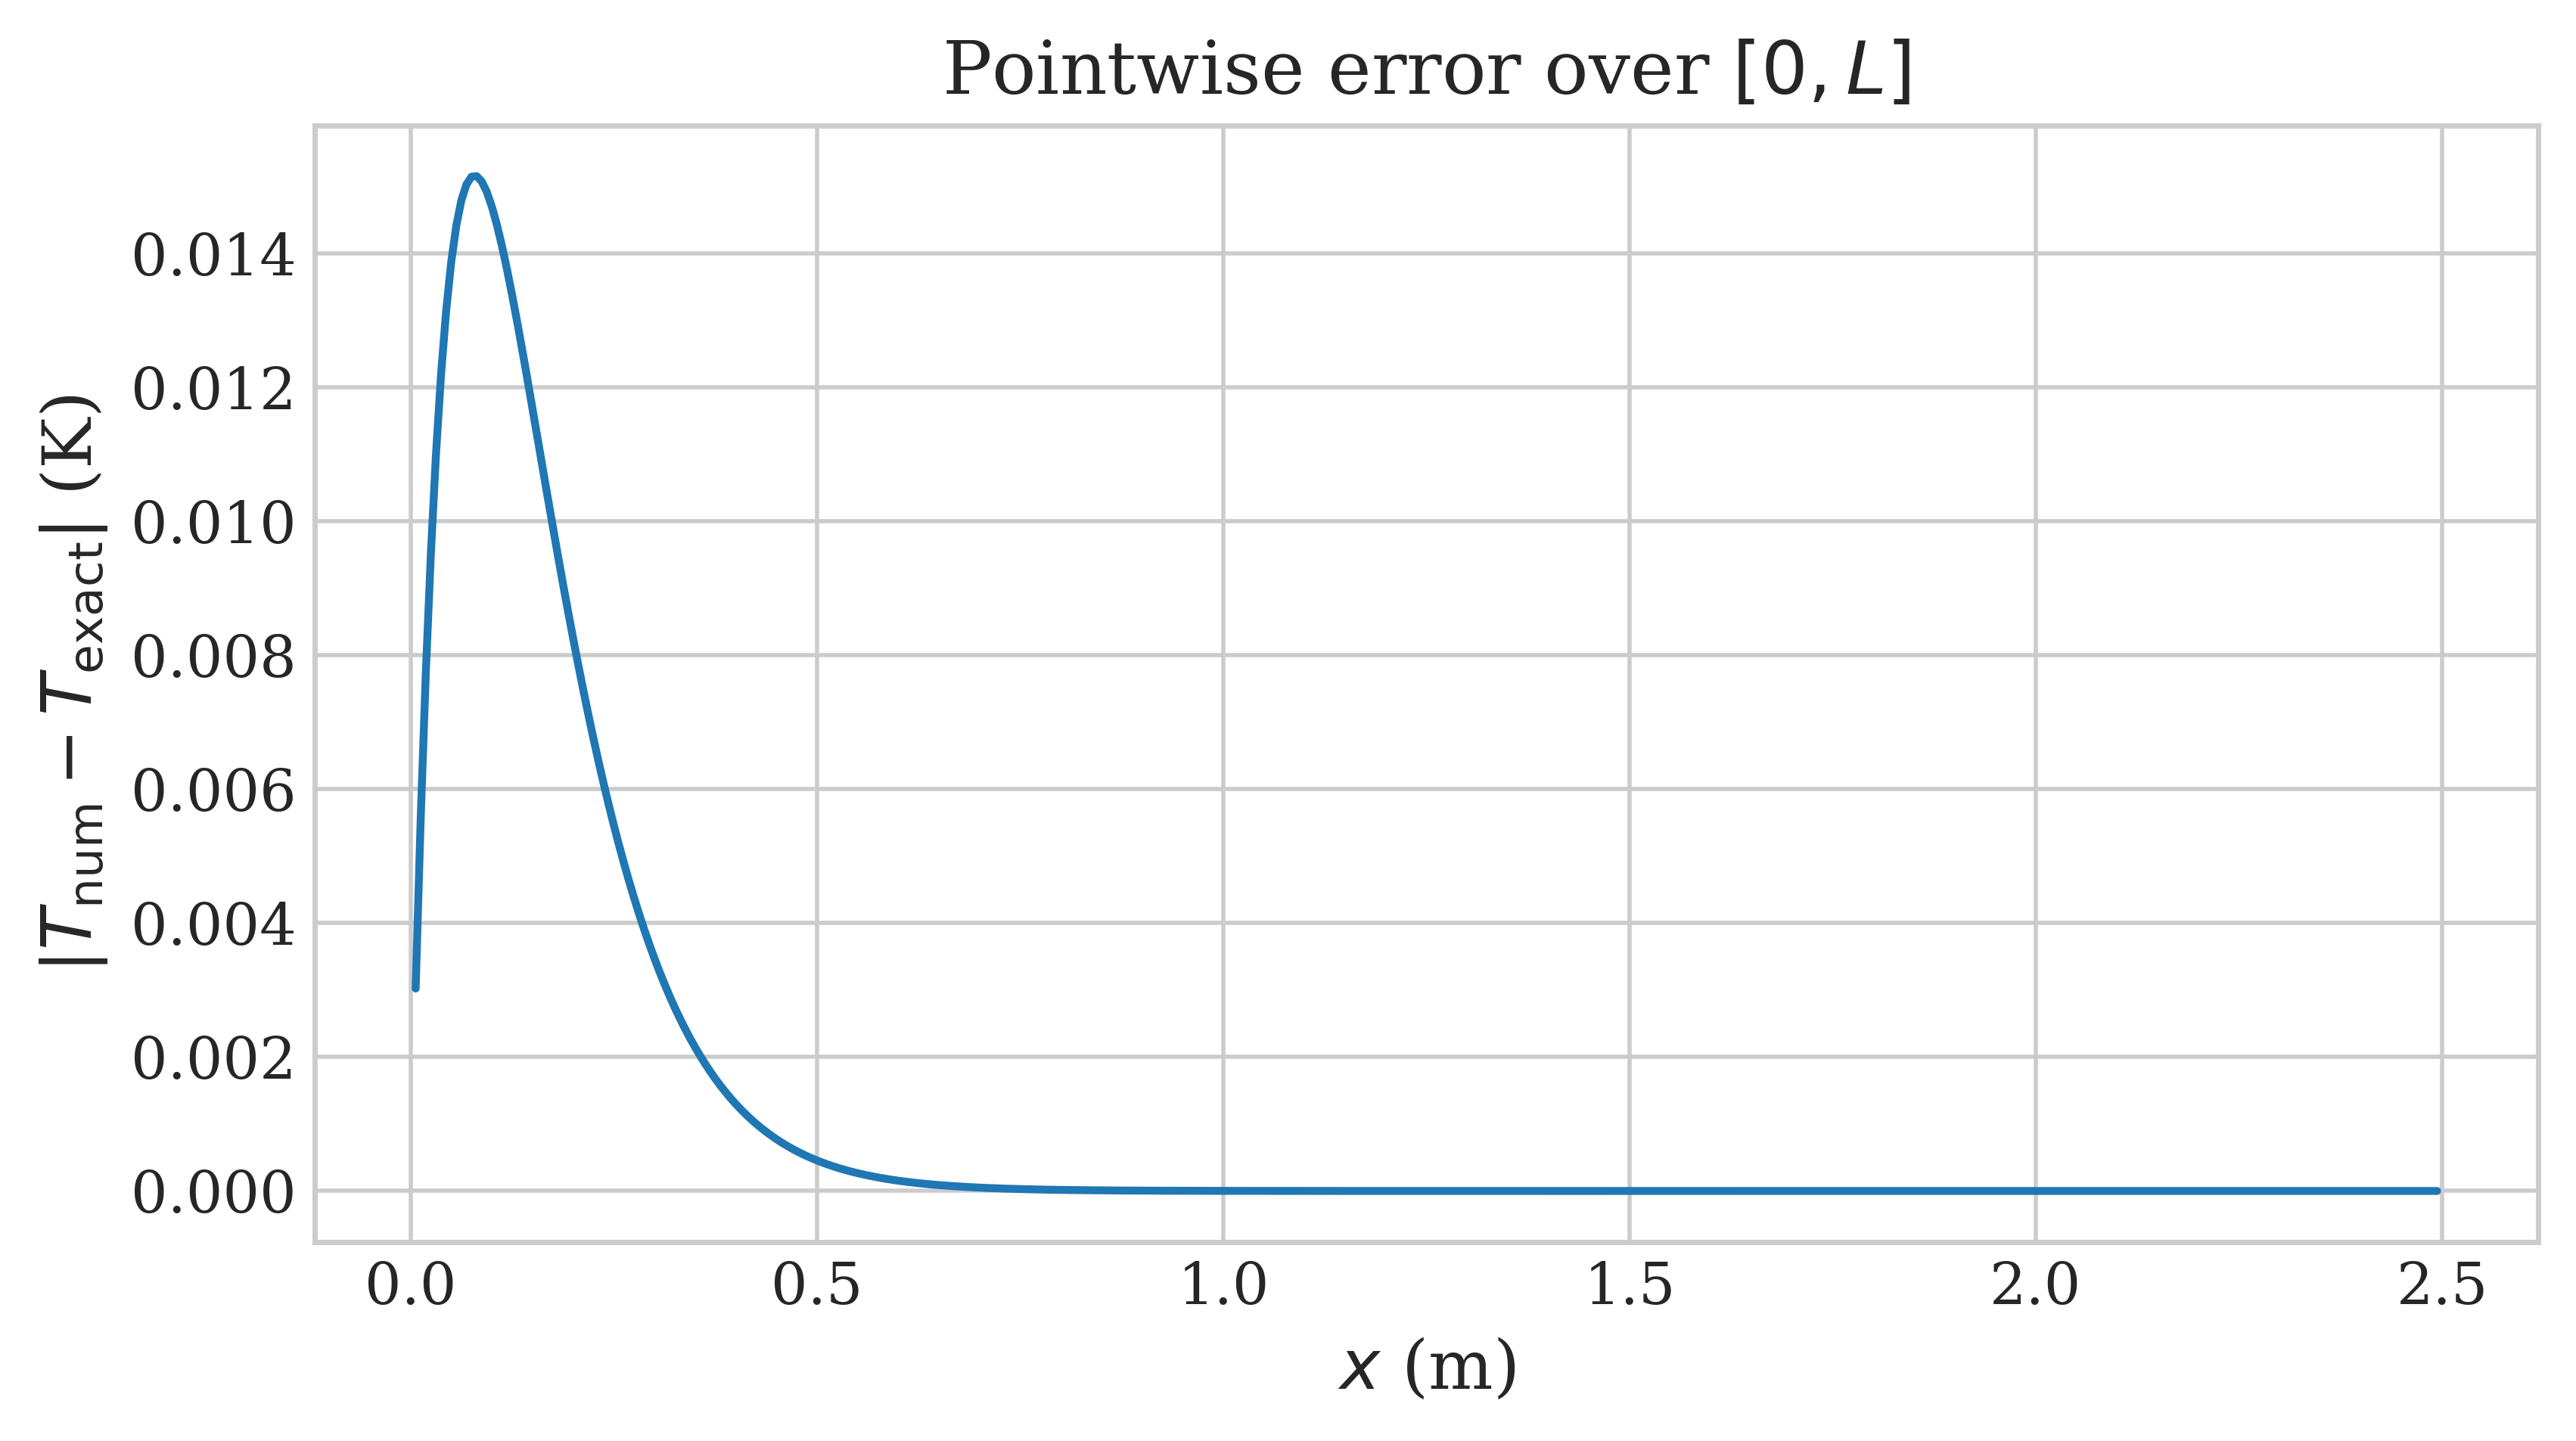
\includegraphics[width=\linewidth]{Plots/8_3a_error.png}
        \caption{Pointwise error of our approximate Newton solution compared to the analytical case \cref{eq:infty-analytical}.}
        \label{fig:heatsink-infty error}
    \end{minipage}
    \hfill
\end{figure}

Judging from \cref{fig:heatsink-inftyT}, the numerical approximation follows the analytical solution closely enough for practical use. For small values of $x$, however, \cref{fig:heatsink-infty error} shows a relatively large bump in the pointwise error. This is a boundary effect: the fixed Dirichlet condition at
$x=0$ makes the first interior node strongly depend on the prescribed value, so the leading $O(h^2)$ error term of a Taylor expansion around this point might still be quite large. As a result, the first "step" away from the boundary is less accurate, even though the method remains globally $O(h^2)$ accurate.

\subsubsection{Method order of accuracy}
Using the same coefficients as in the previous section, we now evaluate the error as a function of $N$. For each $N \in \{50, 100, 200, 400, 800\}$ we solve the boundary value problem numerically and compare the result to the analytical reference solution \cref{eq:infty-analytical}. The discrete 2-norm of the error is defined as
\begin{equation}
\label{eq:2-norm-error}
\|\mathbf{r}\|_2
= \left( \frac{1}{N-1} \sum_{k=1}^{N-1} |r_k|^2 \right)^{1/2},
\end{equation}
where $r_k = T_N(x_k) - T_{\mathrm{ref}}(x_k)$ is the pointwise error
at the interior grid point $x_k$.

To estimate the observed order of accuracy $p$ we use consecutive pairs $(N_{k-1}, N_k)$ and their corresponding errors $e_{N_{k-1}}, e_{N_k}$:
\begin{equation}
\label{eq:order-estimate}
p_k
= \frac{\log\!\left( \dfrac{e_{N_{k-1}}}{e_{N_k}} \right)}
       {\log\!\left( \dfrac{N_k}{N_{k-1}} \right)}.
\end{equation}
If the method is second-order, we expect $p_k \approx 2$ for sufficiently large $N$.

The results are presented in \cref{tab:order-accuracy} and \cref{fig:8.3b-convergence}, the discrete 2-norm $e_N$ decreases approximately like $N^{-2}$, and the estimated orders $p_k$ are close to 2, which confirms that the finite difference method is globally second-order accurate.

\begin{table}[h]
\centering
\begin{tabular}{rccc}
\hline
$N$ & $e_N$ & $p$ \\
\hline
 50  & $2.3051\times 10^{-1}$ & ---    \\
100  & $5.8648\times 10^{-2}$ & $1.9747$ \\
200  & $1.4681\times 10^{-2}$ & $1.9981$ \\
400  & $3.6668\times 10^{-3}$ & $2.0014$ \\
800  & $9.1589\times 10^{-4}$ & $2.0013$ \\
\hline
\end{tabular}
\caption{Discrete 2-norm error $e_N$ and estimated order of accuracy $p$ for different number of intervals $N$.}
\label{tab:order-accuracy}
\end{table}

\begin{figure}[H]
    \centering
    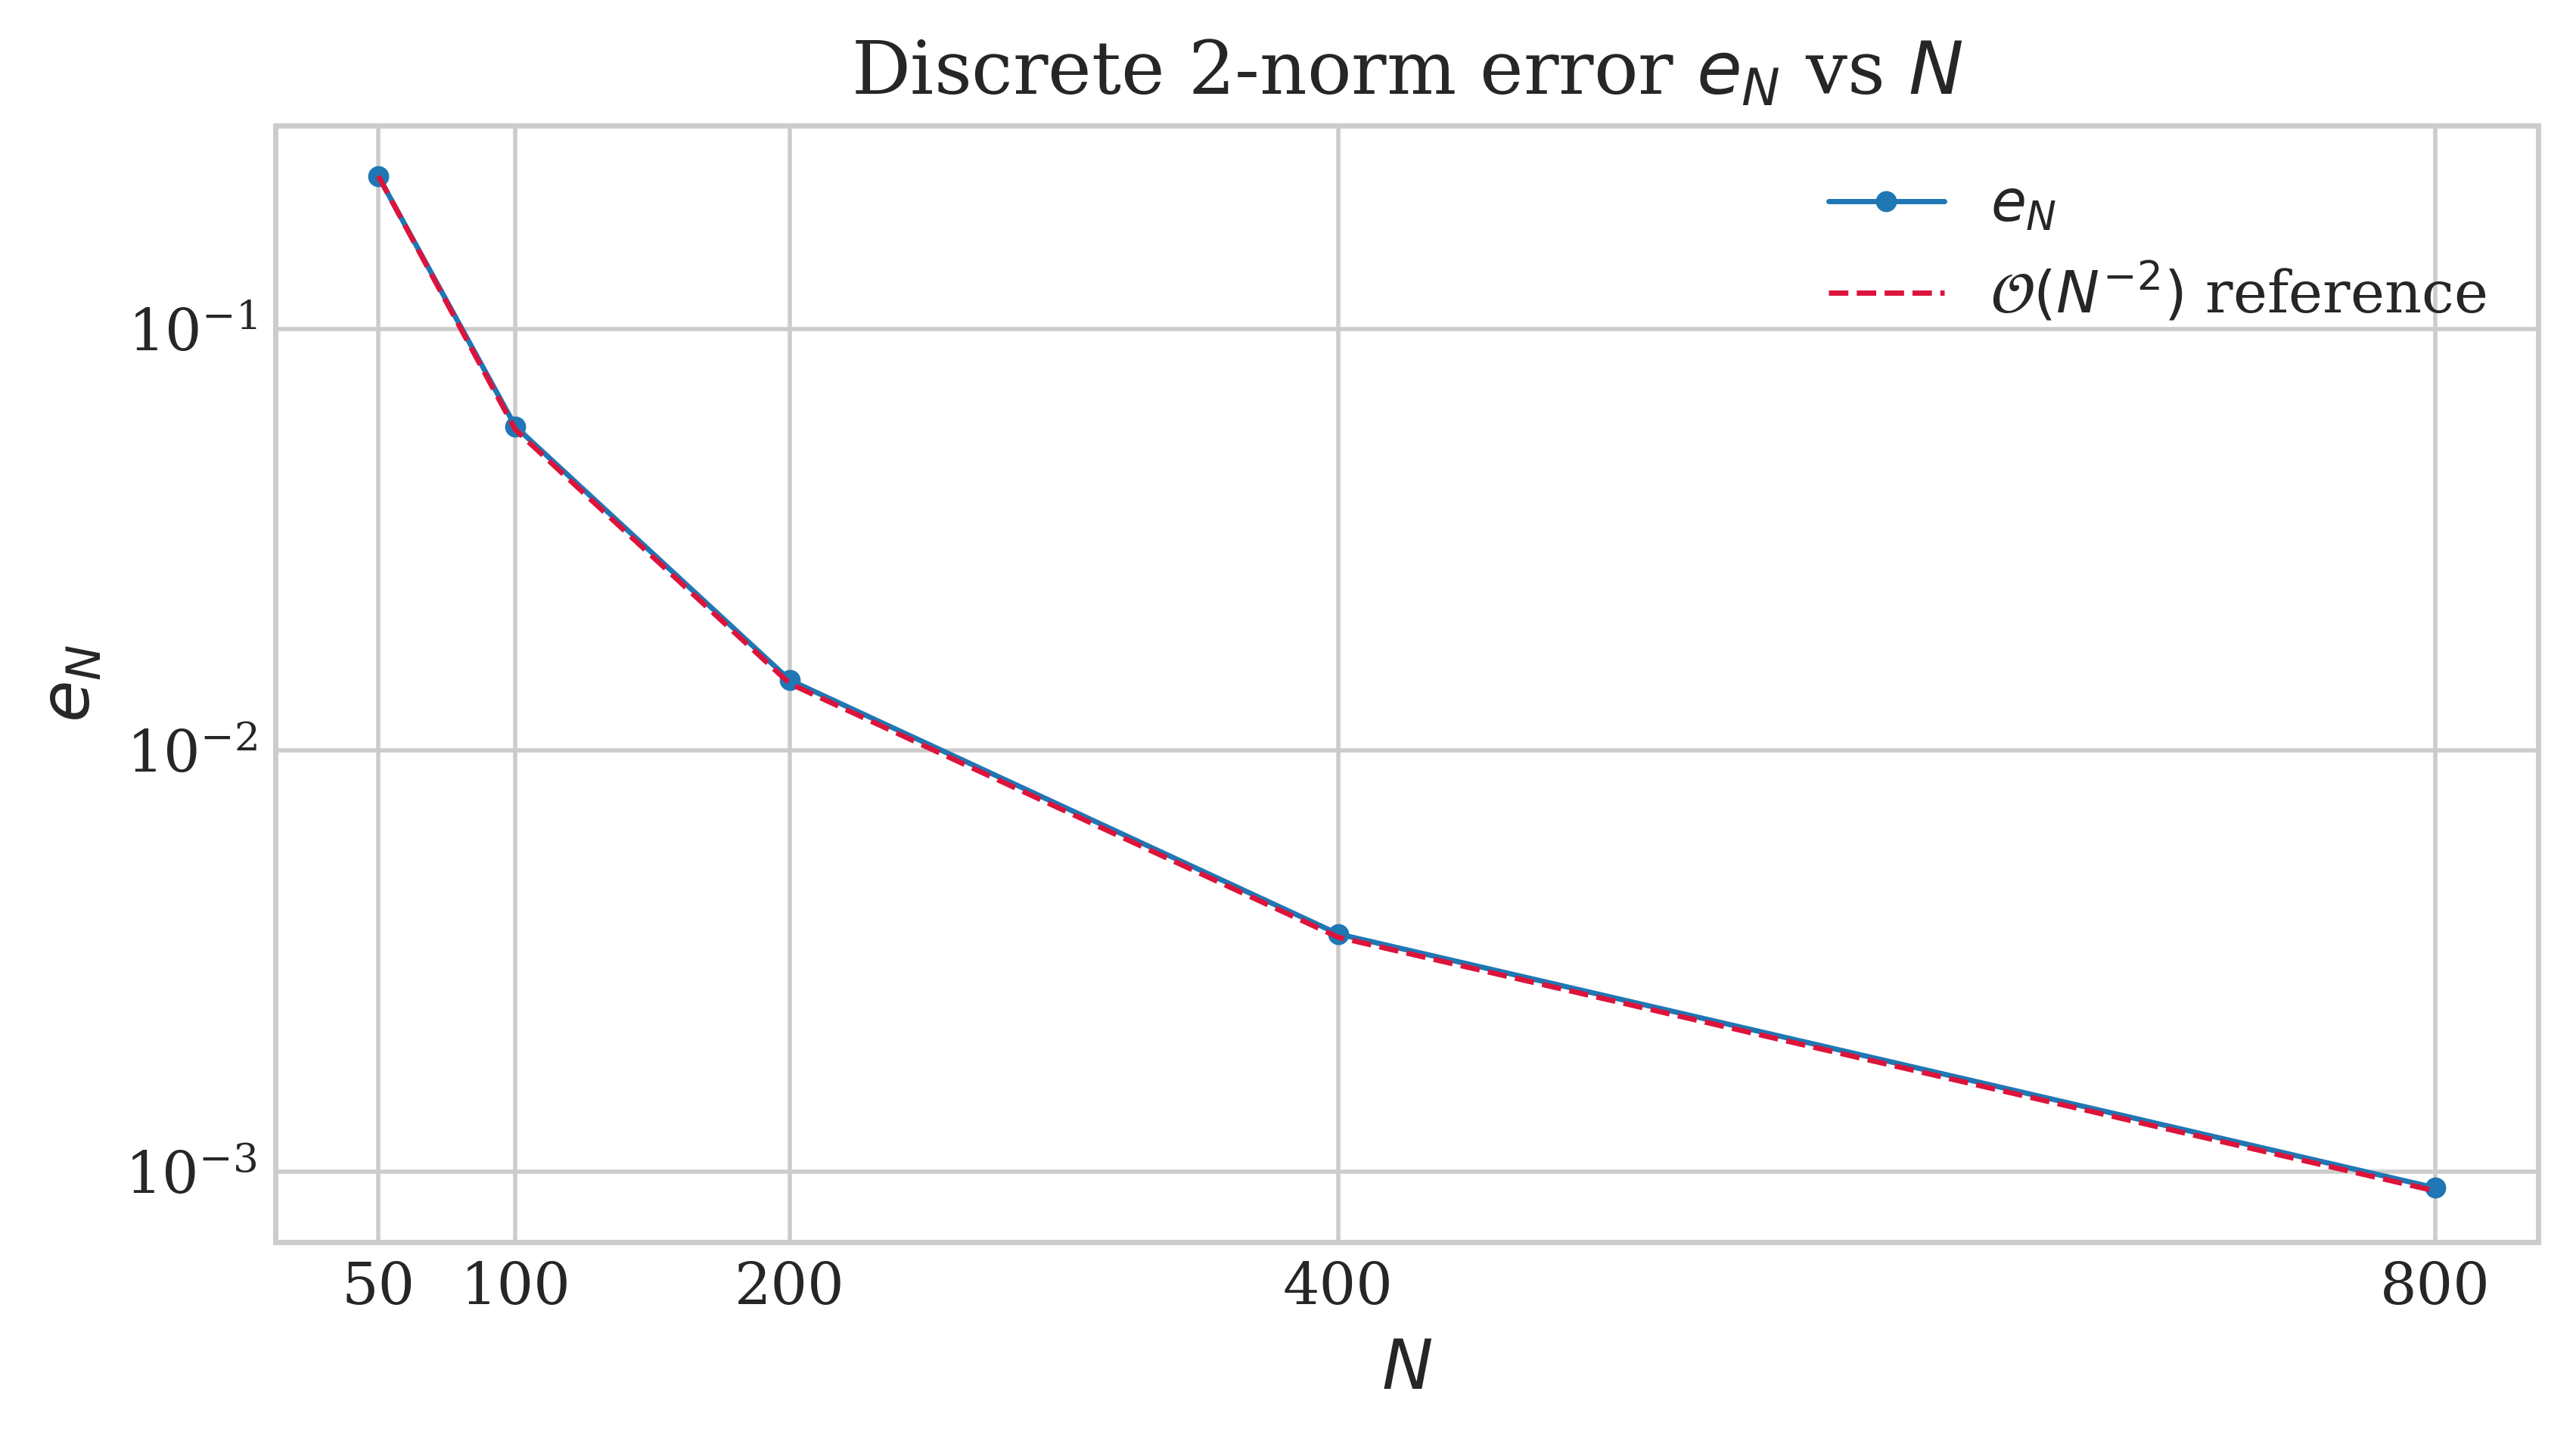
\includegraphics[width=0.75\linewidth]{Plots/8_3b_convergence.png}
    \caption{Discrete 2-norm error as a function of N.}
    \label{fig:8.3b-convergence}
\end{figure}

% ------------------------------------------------------------------------------
\subsubsection{Non-Linear Case: SS AISI 316, Aluminium, and Copper}

We now include the second term ($\alpha_2 \neq 0$) and solve the full
non-linear \cref{eq:heateq} for three materials: stainless steel
(AISI 316), aluminium alloy, and copper.

The geometry and boundary conditions are equal for all materials and is:
$L = 0.30\ \mathrm{m}$,
$D = 5.0\times10^{-3}\ \mathrm{m}$,
$T(0) = 373.15\ \mathrm{K}$,
and $T(L) = T_\infty = 293.15\ \mathrm{K}$.
The material-specific coefficients are

\begin{equation}
  \alpha_1 = \frac{4h_c}{DK}, \qquad \alpha_2 = \frac{4\epsilon\sigma}{DK},
  \label{eq:alpha12}
\end{equation}

with $\sigma$ being Boltzmann's constants\footnote{$\sigma = 5.67\times10^{-8}\ \mathrm{W\,m^{-2}\,K^{-4}}$} and the
remaining parameters taken from \cref{tab:materials}.

\begin{table}[H]
  \centering
  \begin{tabular}{@{}lcccccc@{}}
    \toprule
    Material
      & $K\ \bigl[\frac{\mathrm{W}}{\mathrm{m\,K}}\bigr]$
      & $h_c\ \bigl[\frac{\mathrm{W}}{\mathrm{m^2 K}}\bigr]$
      & $\epsilon$
      & $\alpha_1\ [\mathrm{m}^{-2}]$
      & $\alpha_2\ [\mathrm{m}^{-2}\mathrm{K}^{-3}]$ \\
    \midrule
    SS AISI 316 & $14$  & $100$ & $0.17$
                & $5714.29$
                & $5.508\times10^{-7}$ \\
    Aluminium   & $180$ & $100$ & $0.82$
                & $444.44$
                & $2.066\times10^{-7}$ \\
    Copper      & $398$ & $100$ & $0.03$
                & $201.00$
                & $3.419\times10^{-9}$ \\
    \bottomrule
  \end{tabular}
  \caption{Material parameters and computed coefficients.}
  \label{tab:materials}
\end{table}

Using the code in \cref{lst:heatsinks} with $N = 400$, the temperature
distributions for each material are plotted in \cref{fig:84a-Tx}.

\begin{figure}[H]
  \centering
  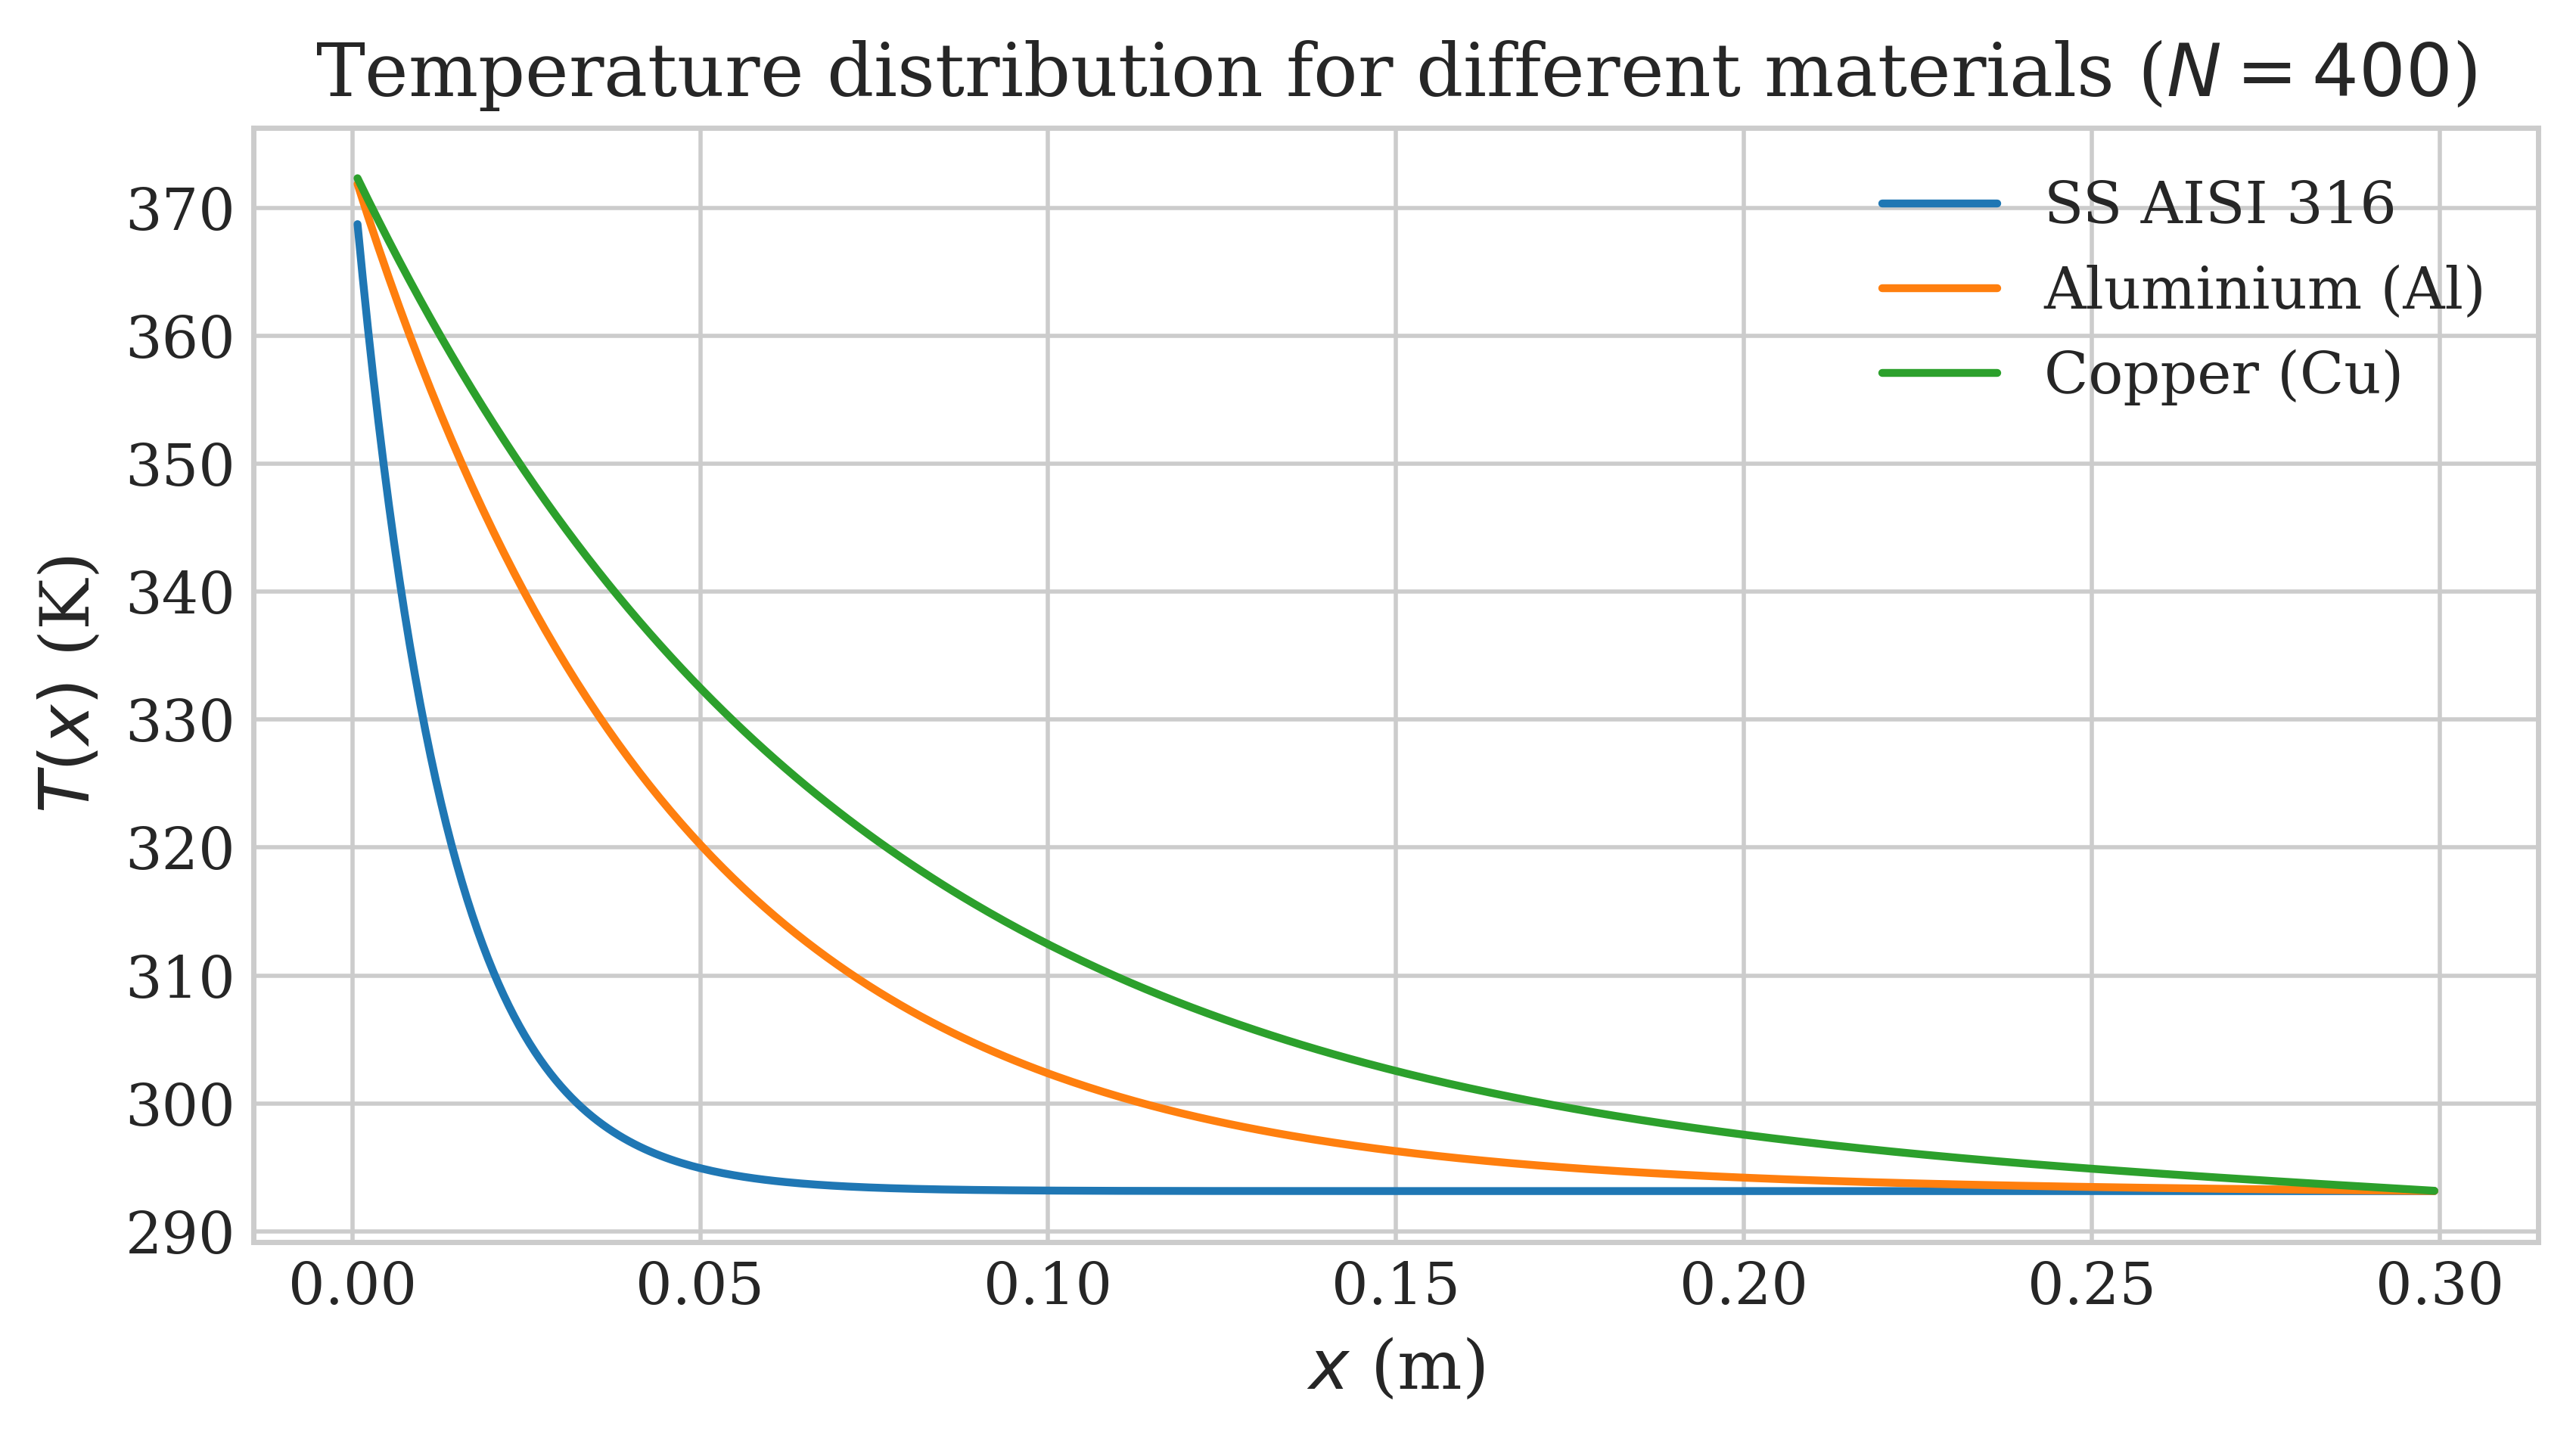
\includegraphics[width=0.72\linewidth]{Plots/8_4a_materials.png}
  \caption{Temperature distribution $T(x)$ along the heat sink for three
  materials, with ($\alpha_2 \neq 0$), $N=400$.}
  \label{fig:84a-Tx}
\end{figure}

The three profiles in \cref{fig:84a-Tx} differ substantially, why that is is evident directly
from $\alpha_1$ in \cref{tab:materials}. Since $\alpha_1 \propto K^{-1}$, a lower thermal conductivity
produces a \textit{larger} $\alpha_1$ and therefore a steeper exponential
decay toward $T_\infty$. The stainless steel drop to near-ambient temperature
within the first few centimeters due to it's poor thermal conductivity.
The aluminum decays more gradually, while the copper disperses the energy the most,
maintaining an elevated temperature almost across the full $0.30\ \mathrm{m}$ length.
$\alpha_2$ plays a minor role here since its values are several orders of
magnitude smaller than $\alpha_1$.

\paragraph{Required length for the infinite assumption.}

The analytical solution for the infinite case (\cref{eq:infty-analytical})
assumes that the temperature decreases exponentially and to an infinitesimal degree approaches the ambient temperature as $x \to \infty$.
If we apply a threshold for when we may say that this approximation is valid, e.g when the deviation is less than $1\%$, we get a practical first estimate of a cut-off length:

\begin{equation}
	e^{-\sqrt{\alpha_1}\,L} < 0.01
	\;\Longleftrightarrow\;
	-\sqrt{\alpha_1}\,L < \ln(0.01)
	\;\Longleftrightarrow\;
	L > \frac{-\ln(0.01)}{\sqrt{\alpha_1}} \approx \frac{4.6}{\sqrt{\alpha_1}}.
	\label{eq:infinite-criterion}
\end{equation}

Applying \cref{eq:infinite-criterion} to each material gives the minimum
lengths in \cref{tab:infinite-length}.

\begin{table}[H]
  \centering
  \begin{tabular}{@{}lccc@{}}
    \toprule
    Material     & $\sqrt{\alpha_1}\ [\mathrm{m}^{-1}]$
                 & $L_{\min} = 4.6/\sqrt{\alpha_1}\ [\mathrm{m}]$
                 & Valid at $L = 0.30\ \mathrm{m}$? \\
    \midrule
    SS AISI 316  & $75.6$ & $0.061$ & Yes \\
    Aluminium    & $21.1$ & $0.218$ & Yes \\
    Copper       & $14.2$ & $0.324$ & \textbf{No} \\
    \bottomrule
  \end{tabular}
  \caption{Minimum length for the infinite-length assumption to hold
  ($< 1\%$ error at the tip).}
  \label{tab:infinite-length}
\end{table}

The stainless steel satisfies the criterion at just $6.1\ \mathrm{cm}$
since its low conductivity traps the majority of energy near the base.
The aluminium requires roughly $22\ \mathrm{cm}$, which is within the simulated $30\ \mathrm{cm}$. And lastly, the copper \textit{does not} satisfy the criterion at $L = 0.30\ \mathrm{m}$: its high
conductivity means the temperature disperses rapidly and well throughout and has not decayed sufficiently by the tip.
Therefore the infinite-length formula \cref{eq:infty-analytical} would underestimate the
tip temperature and overestimate the total heat loss for copper heat sinks of this
length. 

Using \cref{lst:heatsinks} we calculate the full temperature distribution for several lengths for each of the different materials using Newton's Method as described in \cref{solving-the-system}, the results are presented in \cref{fig:T_SS}, \cref{fig:T_Al}, \cref{fig:T_Cu}:


\begin{figure}[h!]
	\centering
	
	\begin{subfigure}{0.60\linewidth}
		\centering
		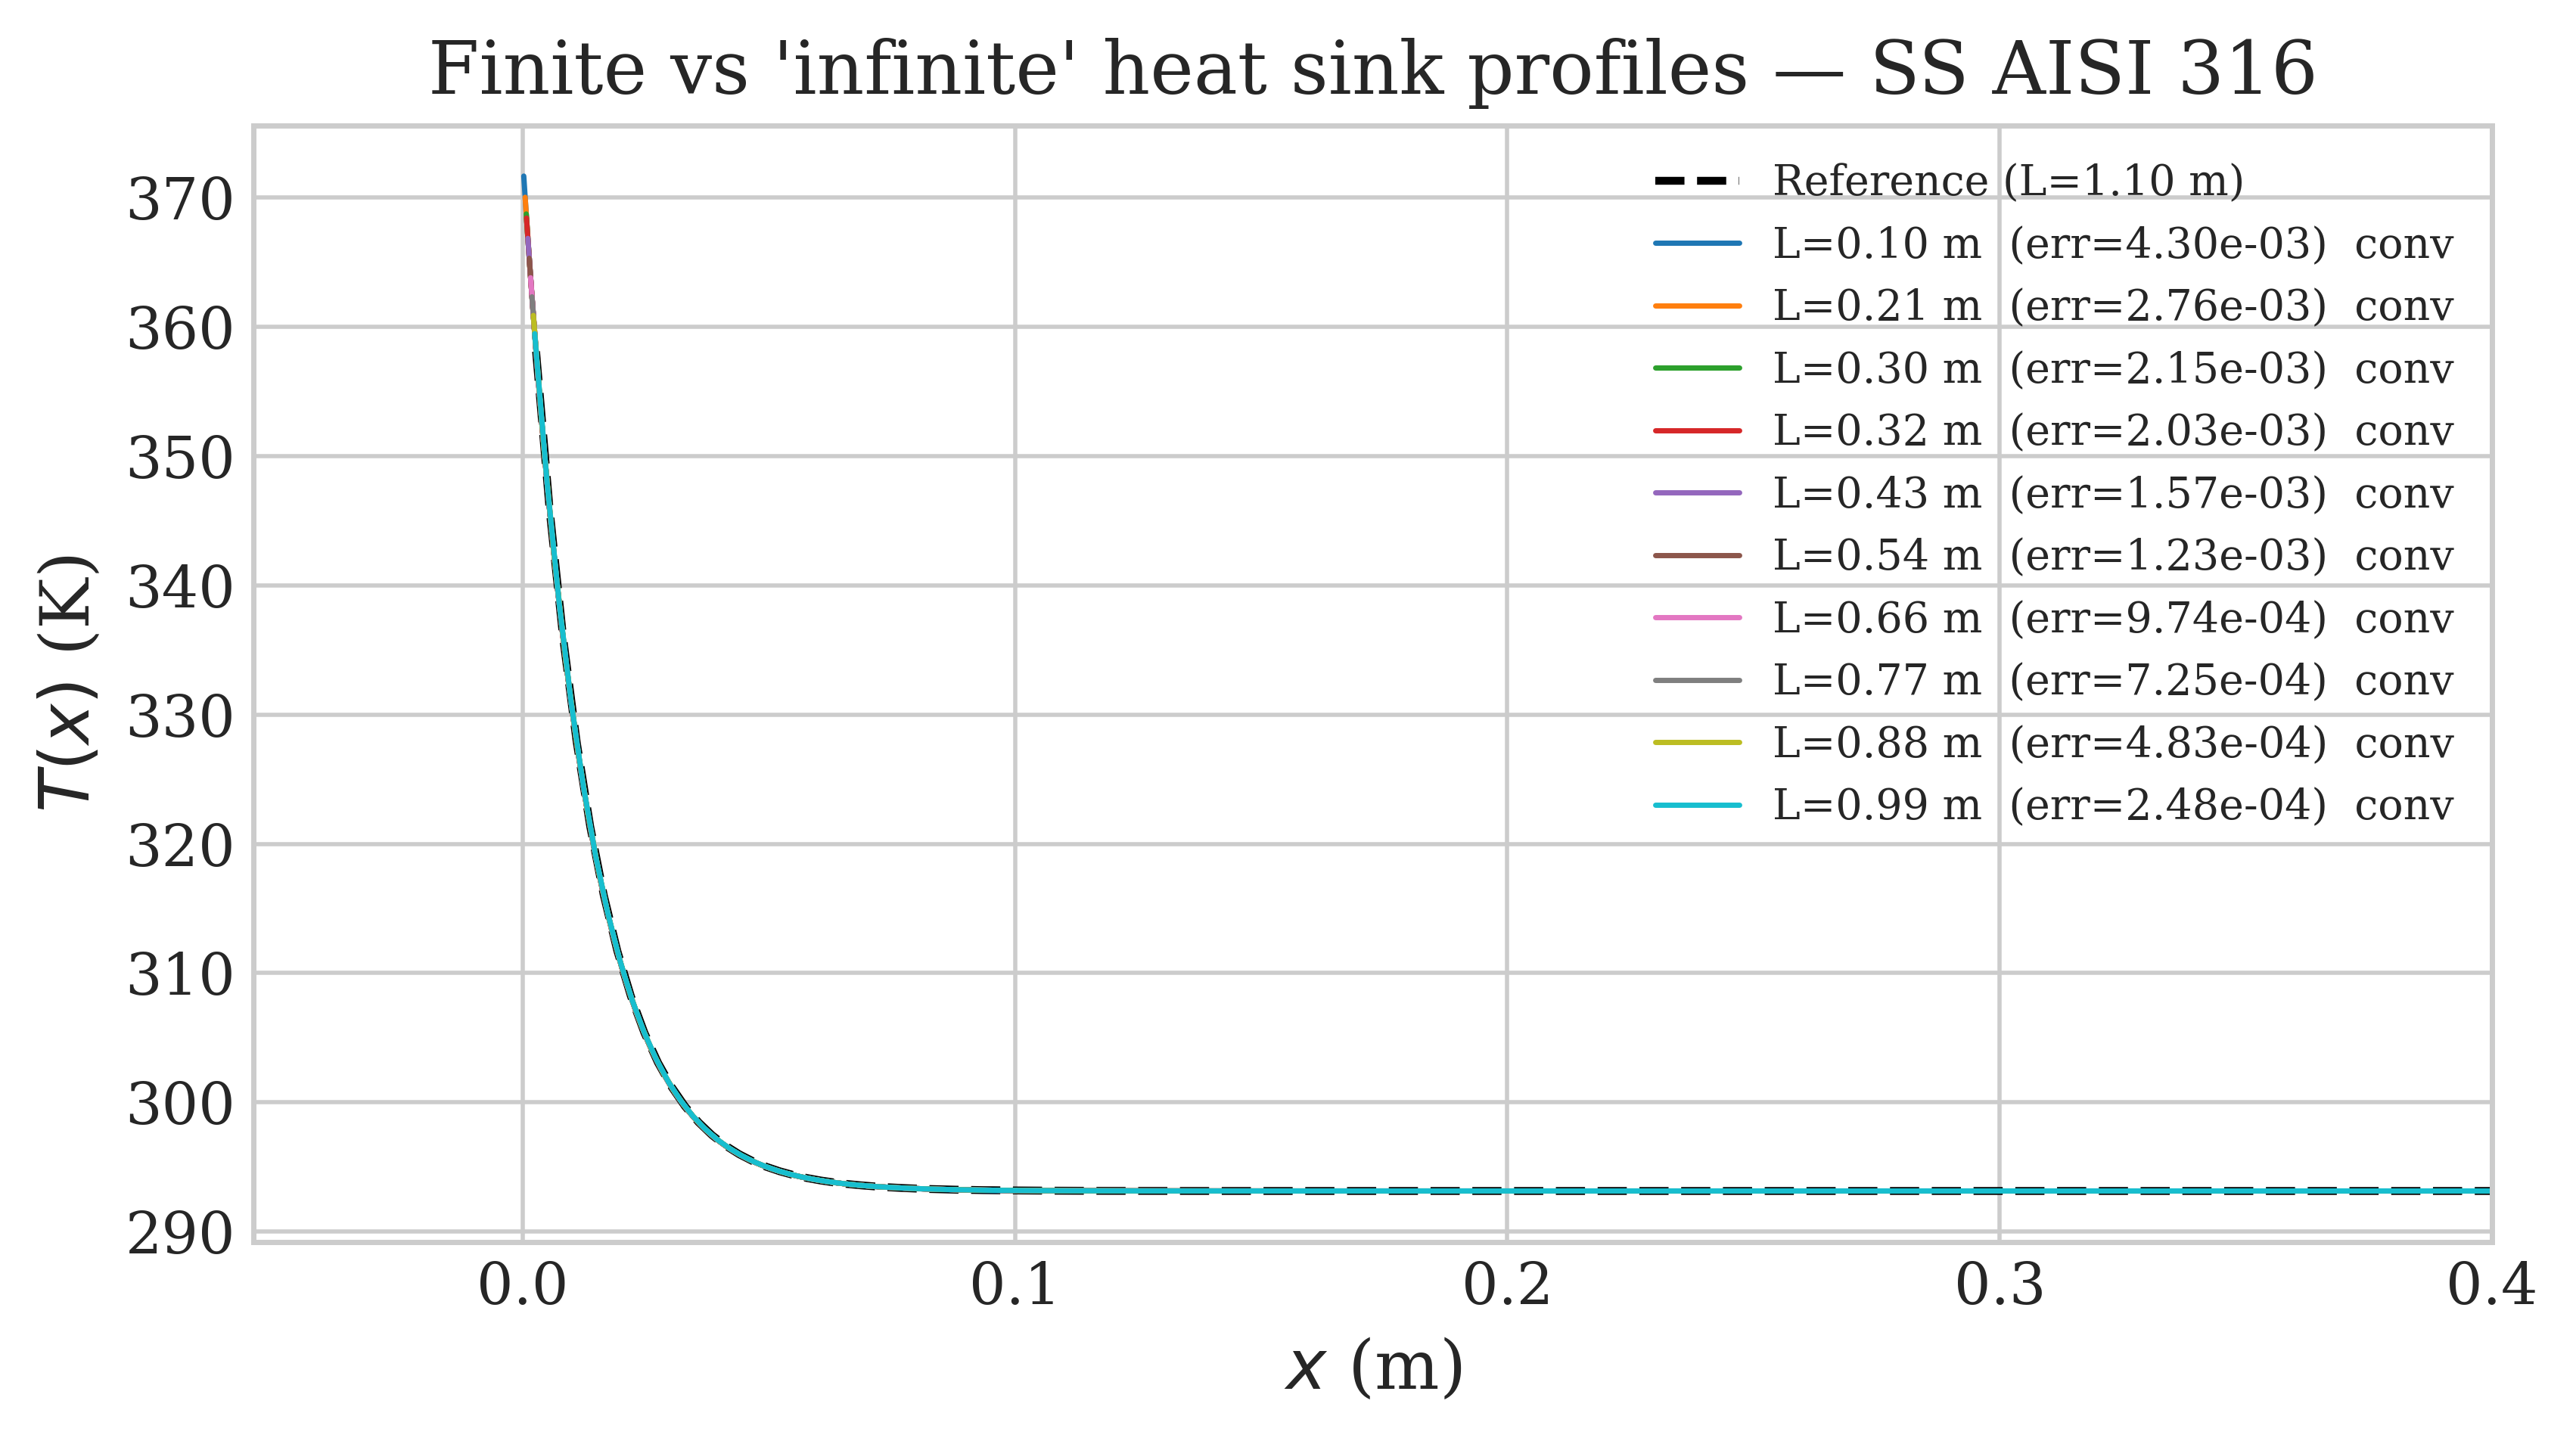
\includegraphics[width=\linewidth]{Plots/8_4b_SS_AISI_316.png}
		\caption{SS AISI 316}
		\label{fig:T_SS}
	\end{subfigure}
	\hfill
	\begin{subfigure}{0.60\linewidth}
		\centering
		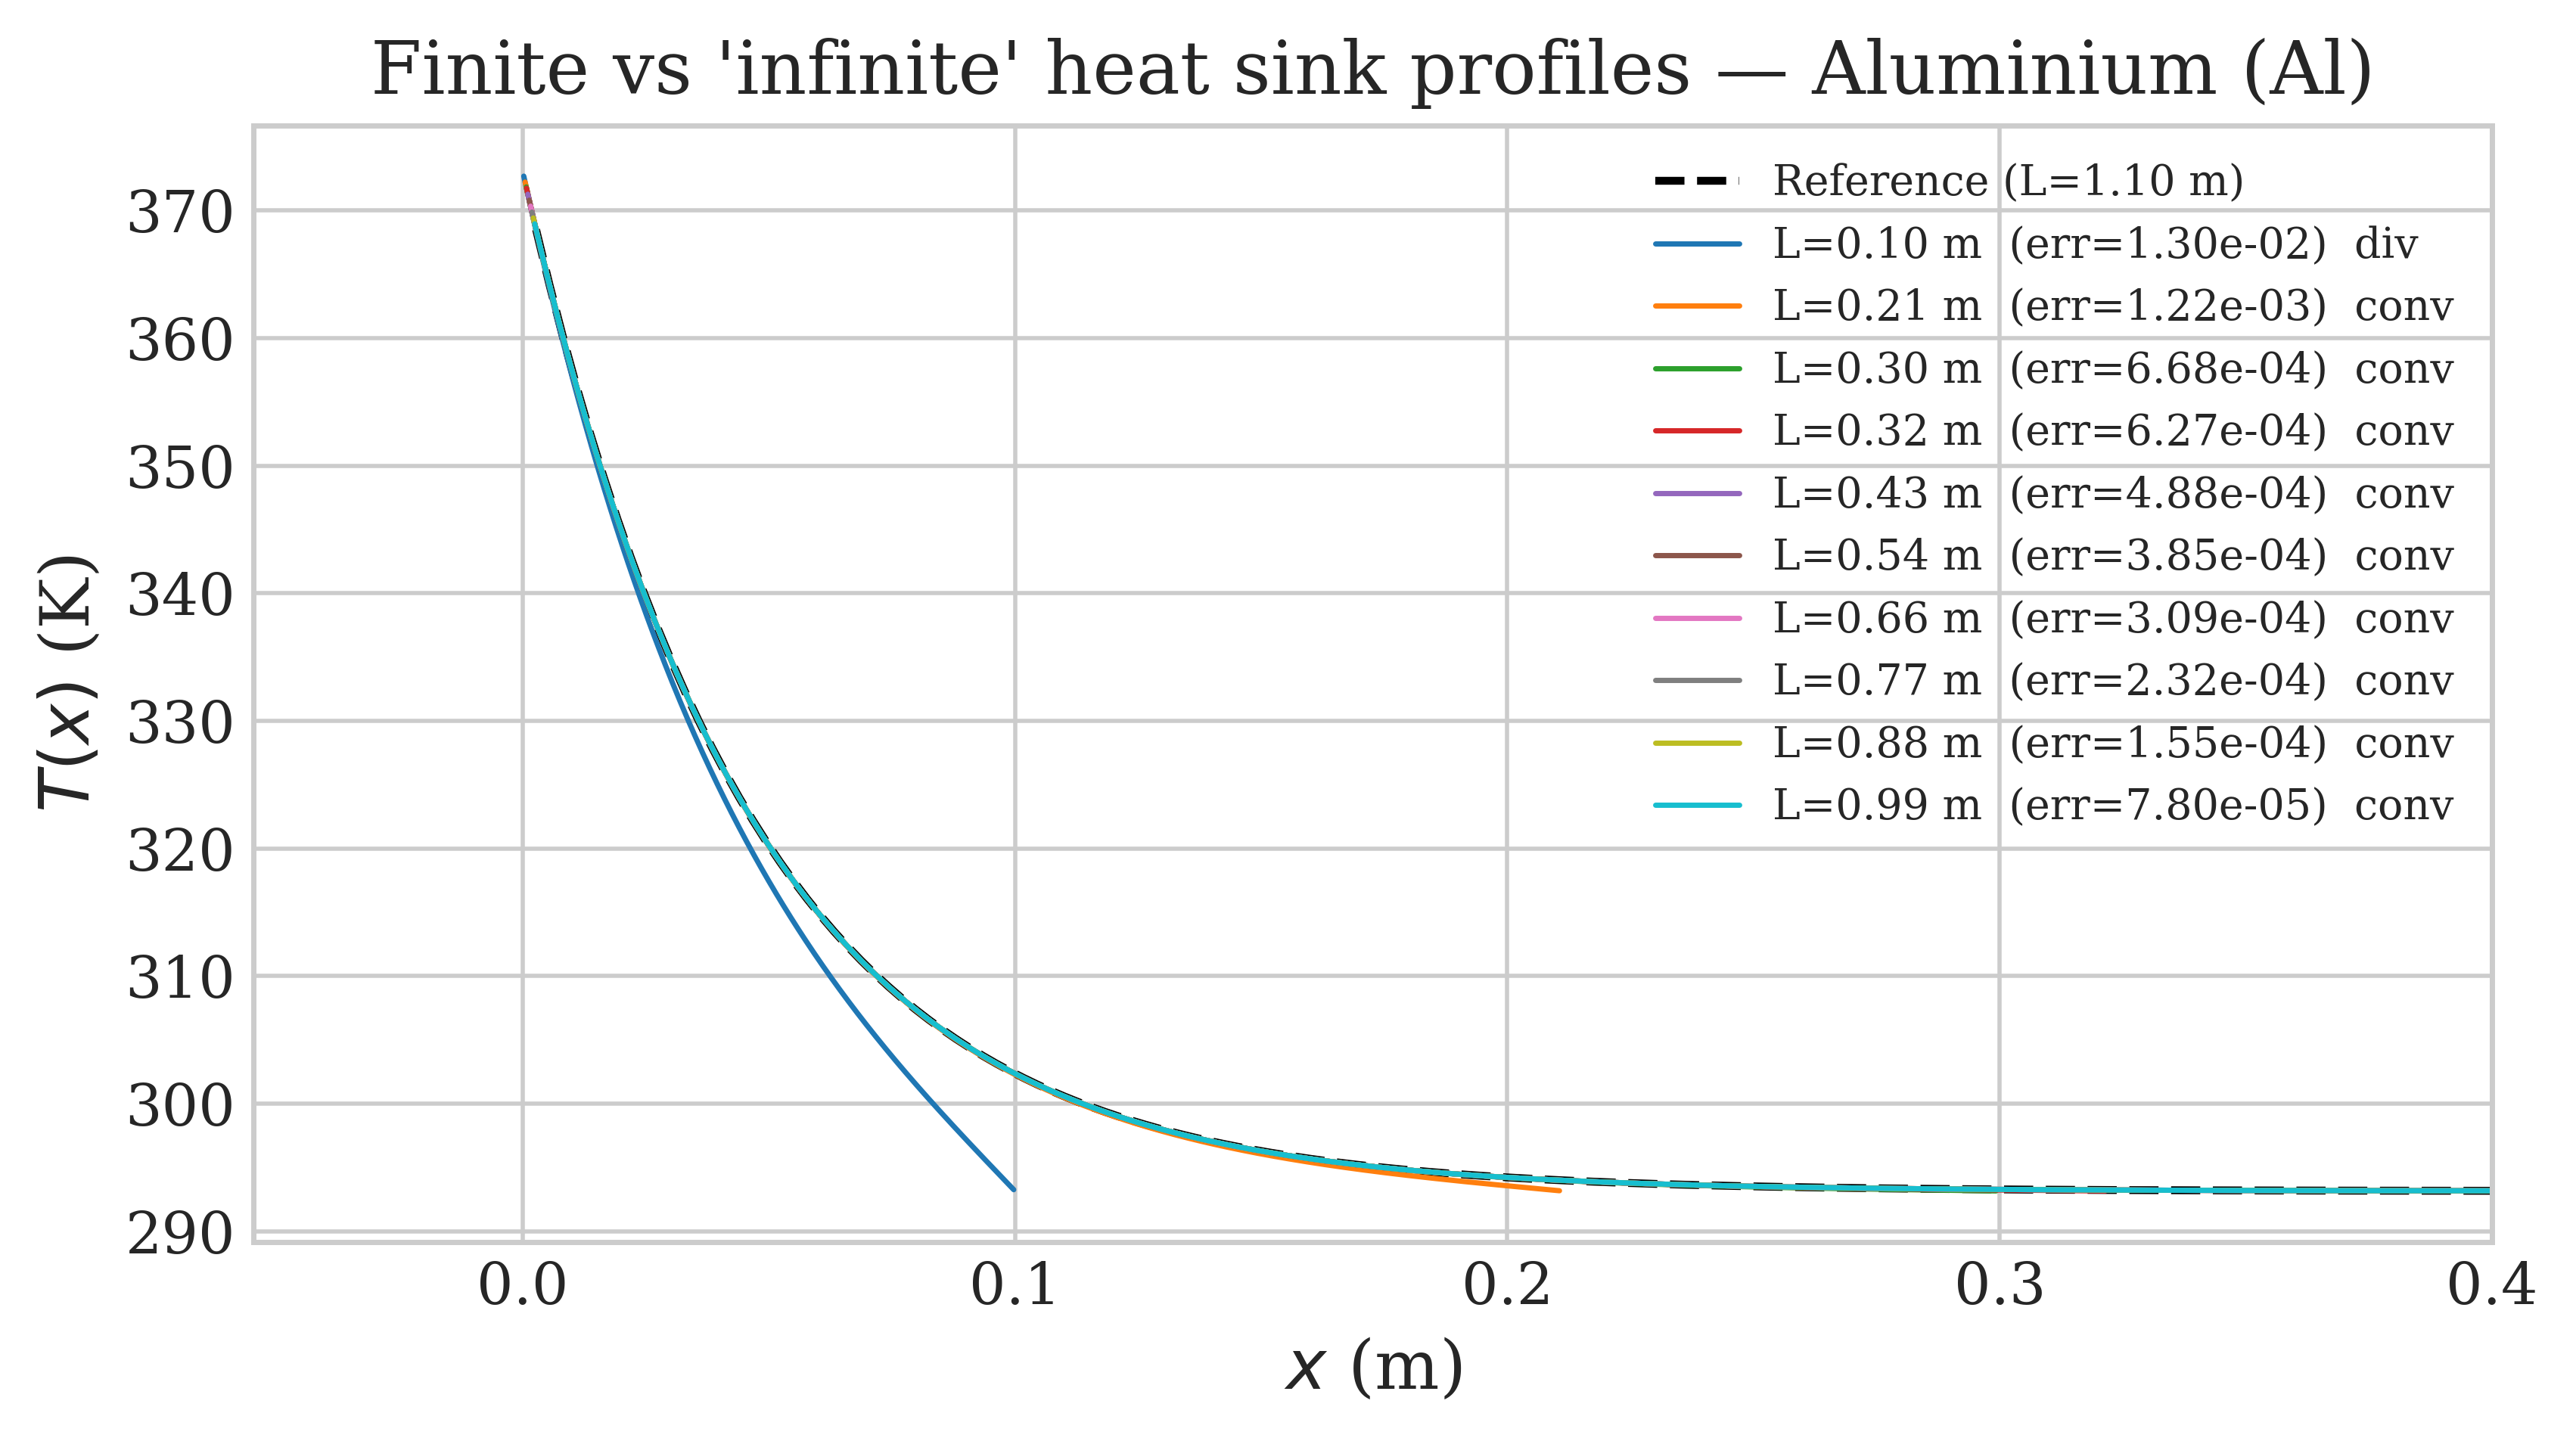
\includegraphics[width=\linewidth]{Plots/8_4b_Aluminium_(Al).png}
		\caption{Aluminium}
		\label{fig:T_Al}
	\end{subfigure}
	\hfill
	\begin{subfigure}{0.60\linewidth}
		\centering
		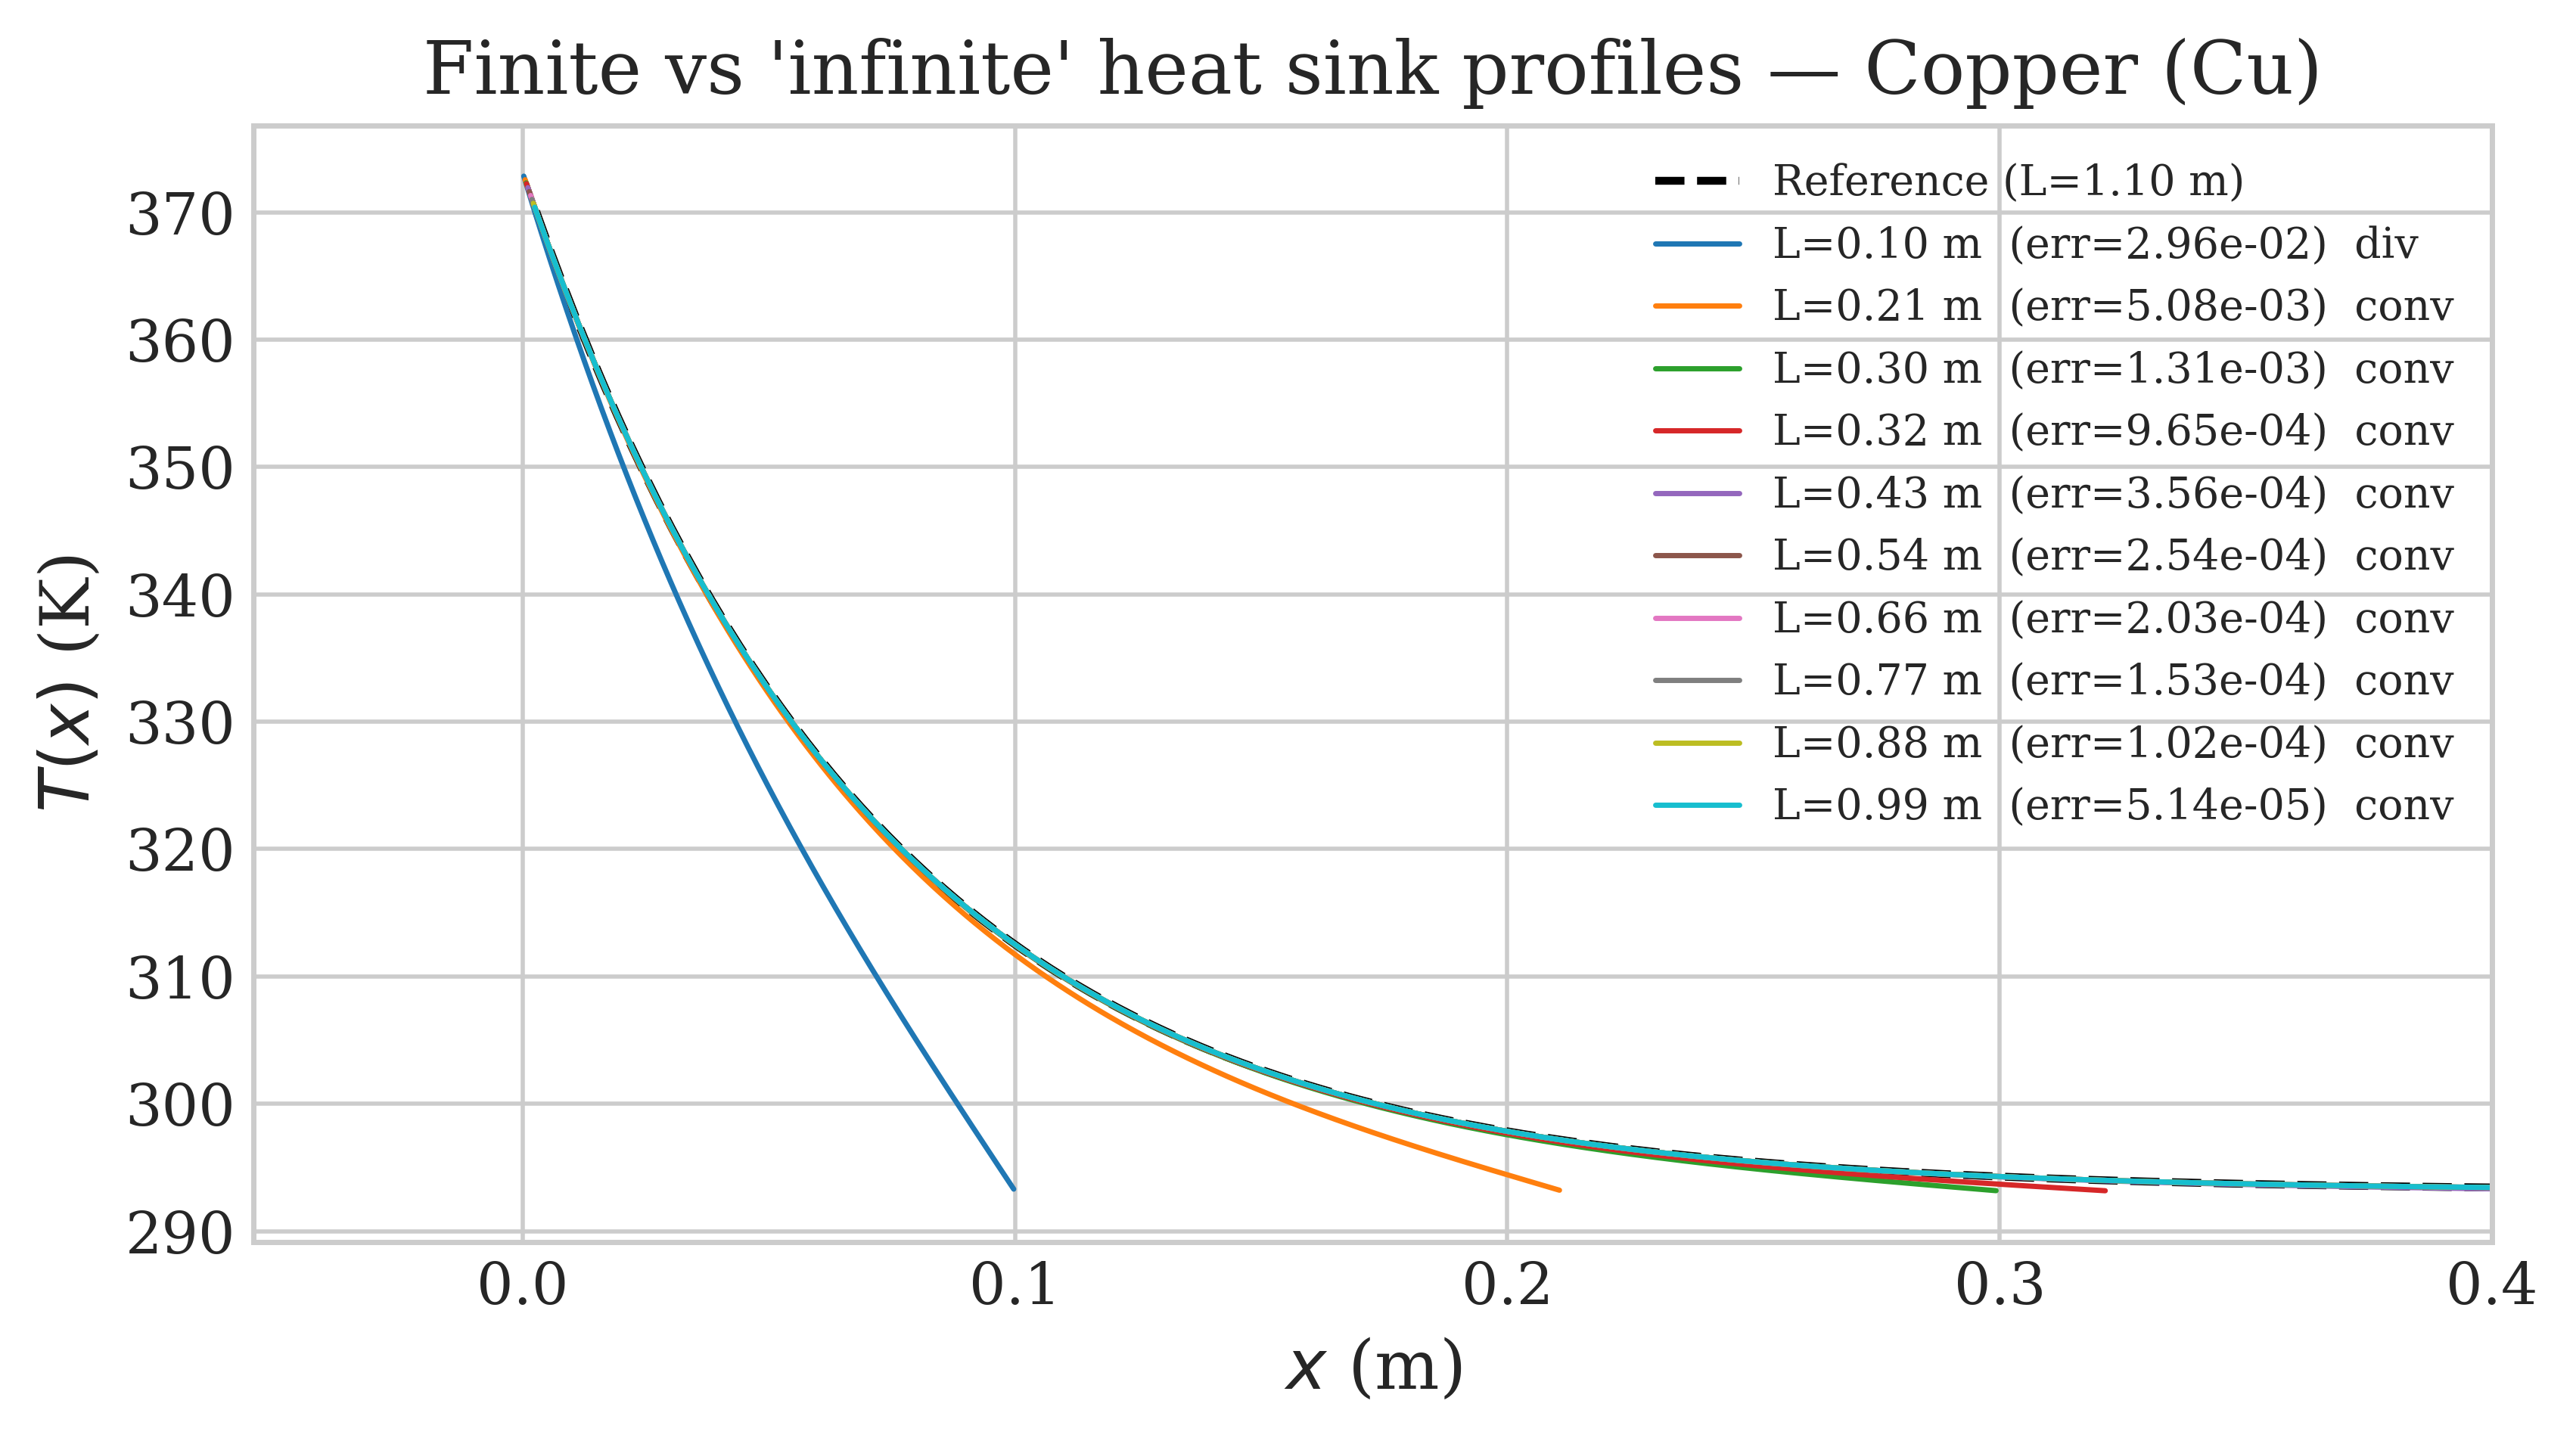
\includegraphics[width=\linewidth]{Plots/8_4b_Copper_(Cu).png}
		\caption{Copper}
		\label{fig:T_Cu}
	\end{subfigure}
	
	\caption{Temperature distribution \(T(x)\) for different materials.}
	\label{fig:T_materials}
\end{figure}
 
% ══════════════════════════════════════════════════════════════════════════════
\section{Discussion}
\newpage
% ── References ────────────────────────────────────────────────────────────────
\begin{thebibliography}{h!}

\end{thebibliography}
\newpage
% ── Appendix ──────────────────────────────────────────────────────────────────
\appendix
\section{Python Source Code}
\label{app:code}

\subsection*{Heat Exchanger -- Newton's Method for non-linear equation}
\lstinputlisting[caption={Heat Exchanger -- Newton's Method for non-linear equation},
                 label={lst:NM-eq}]{Code/newton_non_linear_eq.py}

\subsection*{Heat Exchanger -- Newton's Method for non-linear system}
\lstinputlisting[caption={Heat Exchanger -- Newton's Method for non-linear system},
                 label={lst:NM-sys}]{Code/newton_non_linear_system.py}

\subsection*{Heat Sink -- Newton's Method for non-linear system}
\lstinputlisting[caption={Heat Sink -- Newton's Method for non-linear system},
                 label={lst:heatsinks}]{Code/finite_diff_newton_sys.py}

\subsection*{Structures}
\lstinputlisting[caption={Structures},
                 label={lst:structs}]{Code/structures.py}

\subsection*{Methods}
\lstinputlisting[caption={Methods},
                 label={lst:methods}]{Code/methods.py}

\end{document}